\documentclass{report}
\usepackage{amsmath}
\usepackage{amssymb}
\usepackage[margin=0.75in]{geometry}
\usepackage{fancyhdr}
\usepackage{multirow}
\usepackage{etoolbox}
\usepackage{amsthm}
\usepackage{tikz,pgfplots}
\usepackage{stackengine}
\usepackage{tcolorbox}
\usetikzlibrary{arrows}
\usepackage{array,booktabs,arydshln,xcolor}
\usepgfplotslibrary{fillbetween}
\pgfplotsset{compat=1.16,width=10cm}

\parskip = 0.2in
\setlength\parindent{24pt}


%%Section and chapter references macros
%%%%%%%%%%%%%%%%%%%

\makeatletter
\newcommand*{\currentname}{\@currentlabelname}
\makeatother

\newcommand\getcurrentref[1]{%
 \ifnumequal{\value{#1}}{0}
  {??}
  {\the\value{#1}}%
}    

%%%%%%%Commands%%%%%%%%%%%%%%%%%%%%%
\theoremstyle{definition}
\newtheorem{example}{\bf Example}
\newtheorem{definition}{\bf Definition}[section]
\newtheorem{youtry}{\textbf{You Try It!}}
\newtheorem{step}{\textbf{Step}}


%%%%%%%%%%%%%Header%%%%%%%%%%%%%%%%%%%
\pagestyle{fancy}
\fancyhf{}
\renewcommand{\headrulewidth}{0pt}
\lhead{}
\rhead{Algebra 2: Section  \getcurrentref{chapter}.\getcurrentref{section}}
\cfoot{ }
\rfoot{Page \thepage}
%%%%%%%%%%%%%%%%%%%%%%%%%%%%%%%%%%%%%%

%% Set start page here 
\setcounter{page}{1}



%%% Set Chapter counter here
\setcounter{chapter}{5}
\setcounter{section}{0}


%%%%%%%%%%%%%%% New Section Template %%%%%%%%%%%%%%%%
%%%%%%%%%%%%%%%%%%%%%%%%%%%%%%%%
%%%%%%%%%%%%%%%%%%%%%%%%%%%%%%%%
%%%%%%%   Section _._   %%%%%%%%
%%%%%%%%%%%%%%%%%%%%%%%%%%%%%%%%
%%%%%%%%%%%%%%%%%%%%%%%%%%%%%%%%
% \section{    NAME HERE   }
% \setcounter{example}{0}
% \setcounter{definition}{0}
% %%%%%%%%%%%%%%%%%%%%%%%%%%%%%%%%
% %%%%%%%%%%%%%%%%%%%%%%%%%%%%%%%%
% \begin{definition}
%     Definition
% \end{definition}
% \begin{example}
%     Example
% \end{example}
%
%\vspace{-0.5cm}
%\hspace{-0.5cm}
%%
%% LeftOfPage%%%%%
%\begin{minipage}{0.45\linewidth}
% \begin{itemize}
%     \item[(a)]
% \end{itemize}
%%
%\vspace{2.75cm}
%%
% \begin{itemize}
%     \item[(c)]
% \end{itemize}
%%
%\vspace{2.75cm}
%%
%\end{minipage}
%\hspace{1.5cm}
%%RightOfPage%%%%%
%\begin{minipage}{0.45\linewidth}
% \begin{itemize}
%     \item[(b)]
% \end{itemize}
%%
%\vspace{2.75cm}
%%
% \begin{itemize}
%     \item[(d)]
% \end{itemize}
%%
%\vspace{2.75cm}
%%
%\end{minipage}
%%%%%%%%%%%%%%%%%%%%%%
%
%%%%%%%%%%%%%%%%% Example 2
%\begin{example}
%     Use \textbf{elimination} to solve each system of equations.
%\end{example}
%%
%\vspace{-0.5cm}
%\hspace{-0.5cm}
%%
%% LeftOfPage%%%%%
%\begin{minipage}{0.45\linewidth}
% \begin{itemize}
%     \item[(a)]
% \end{itemize}
%%
%\vspace{2.75cm}
%%
% \begin{itemize}
%     \item[(c)]
% \end{itemize}
%%
%\vspace{2.75cm}
%%
%\end{minipage}
%\hspace{1.5cm}
%%RightOfPage%%%%%
%\begin{minipage}{0.45\linewidth}
% \begin{itemize}
%     \item[(b)]
% \end{itemize}
%%
%\vspace{2.75cm}
%%
% \begin{itemize}
%     \item[(d)]
% \end{itemize}
%%
%\vspace{2.75cm}
%%
%\end{minipage}
%%%%%%%%%%%%%%%%%%%%%
%\vfill
% \noindent\fbox{\large\textbf{_._ Homework}: page \small }
%%%%%%%%%%%%%%%%%%%%%%%%%%%%%%%%%%%%%%
%%%%%%%%%%%%%%%%%%%%%%%%%%%%%%%%%%%%%%
% \newpage
%%%%%%%%%%%%%%%%%%%%%%%%%%%%%%%%%%%%%%
%%%%%%%%%%%%%%%%%%%%%%%%%%%%%%%%%%%%%%



% number line example%%%%
%\begin{tikzpicture}
        %\draw[latex-latex] (-3.5,0) -- (3.5,0) ; %edit here for the axis
        %\foreach \x in  {-3,-2,-1,0,1,2,3} % edit here for the vertical lines
        %\draw[shift={(\x,0)},color=black] (0pt,3pt) -- (0pt,-3pt);
        %\foreach \x in {-3,-2,-1,0,1,2,3} % edit here for the numbers
        %\draw[shift={(\x,0)},color=black] (0pt,0pt) -- (0pt,-3pt) node[below] 
        %{$\x$};
        %\draw[*-o] (0.92,0) -- (2.08,0);
        %\draw[very thick] (0.92,0) -- (1.92,0);
%\end{tikzpicture}






\begin{document}


\noindent\LARGE\textbf{Chapter 5 Quadratic Functions}\normalsize

%%%%%%%%%%%%%%%%%%%%%%%%%%%%%%%
%%%%%%%%%%%%%%%%%%%%%%%%%%%%%%%
%%%%%%   Section 5.1   %%%%%%%%
%%%%%%%%%%%%%%%%%%%%%%%%%%%%%%%
%%%%%%%%%%%%%%%%%%%%%%%%%%%%%%%
 \section{Using Transformations to Graph Quadratic Functions }
 \setcounter{example}{0}
 \setcounter{definition}{0}
 \setcounter{youtry}{0}
 %%%%%%%%%%%%%%%%%%%%%%%%%%%%%%%%
 %%%%%%%%%%%%%%%%%%%%%%%%%%%%%%%%
 \hfill \underline{Objective}: Transform quadratic functions. Use the vertex form to graph quadratics.\\
 
 \begin{definition}
 A \textbf{quadratic function} is a function that can be written in the form $f(x)=ax^2+bx+c$ where $a\neq 0$. A graph of the quadratic parent function is shown below. Fill in the table below using a graphing calculator.
 \end{definition}
 
 \vspace{-0.5cm}
 \hfill
 \begin{minipage}[t]{0.45\linewidth}
	 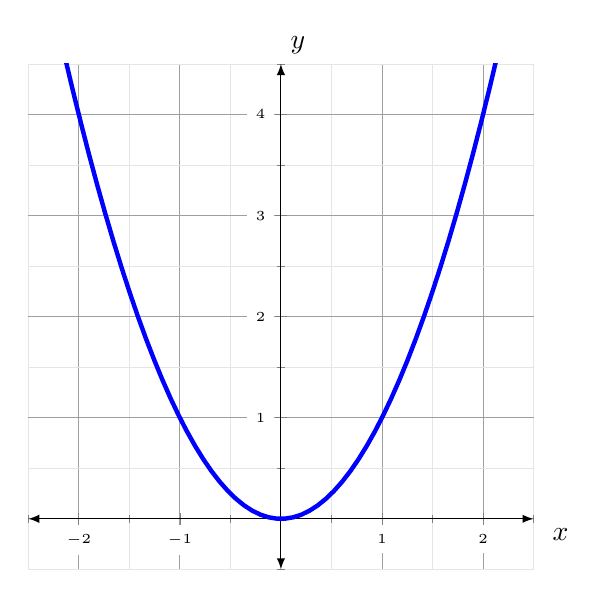
\begin{tikzpicture}[>=triangle 45,]
			\begin{axis}[
					    width =8cm,
				               height=8cm,
					    xmin=-2,xmax=2,
					    ymin=0,ymax=4,
					    grid=both,
					    grid style={line width=.15pt, draw=gray!20},
					    major grid style={line width=.3pt,draw=gray!75},
					    axis lines=middle,
					    minor tick num=1,
					    enlargelimits={abs=0.5},
					    axis line style={latex-latex},
					    ticklabel style={font=\tiny,fill=white},
					    xlabel={\,\,$x$},
					    ylabel={$y$},
					    xlabel style={below right},
					    ylabel style={above right},
					    domain=-4:4,
					]
					\addplot+[<->, blue, ultra thick,samples=100, mark=none ] {x^2};
			\end{axis}
			%\draw[color=blue,thick] plot (\x,\x*\x);
	\end{tikzpicture}
\end{minipage}
\begin{minipage}[t]{0.35\linewidth}
	\large
	\vspace{-6.5cm}
	 \begin{tikzpicture}
	 	%%  T-Chart  %%%%%%%%
		\draw (6,5) --(6,0.5);
		\draw (5.5,4.5) node[above]{$x$} (6.5, 4.5) node[above]{$y_1$};
		\draw (5, 4.5) -- (7, 4.5);
		\draw (5.5, 4) node{$-2$};
		\draw (5.5, 3.25) node{$-1$};
		\draw (5.5, 2.5) node{$0$};
		\draw (5.5, 1.75) node{$1$};
		\draw (5.5, 1) node{$2$};
		%%%%%%%%%%%%%%%
	\end{tikzpicture}
	\normalsize
\end{minipage}

\vfill
\begin{example}
Graph using a graphing calculator table.
\end{example}

\begin{minipage}[t]{0.45\linewidth}
 (a) \,\, $f(x)=x^2-6x+8$\\
\end{minipage}
\hfill
\begin{minipage}[t]{0.4\linewidth}
 (b) \,\, $f(x)=-x^2+6x-8$\\
\end{minipage}

 \begin{minipage}[t]{0.3\linewidth}
	 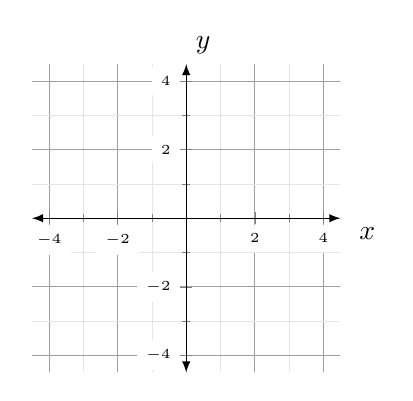
\begin{tikzpicture}[>=latex]
			\begin{axis}[
					    width =5.5cm,
				               height=5.5cm,
					    xmin=-4,xmax=4,
					    ymin=-4,ymax=4,
					    grid=both,
					    grid style={line width=.15pt, draw=gray!20},
					    major grid style={line width=.3pt,draw=gray!75},
					    axis lines=middle,
					    minor tick num=1,
					    enlargelimits={abs=0.5},
					    axis line style={latex-latex},
					    ticklabel style={font=\tiny,fill=white},
					    xlabel={\,\,$x$},
					    ylabel={$y$},
					    xlabel style={below right},
					    ylabel style={above right},
					]
			\end{axis}
			%\draw[color=blue,thick] plot (\x,\x*\x);
	\end{tikzpicture}
\end{minipage}
\begin{minipage}[t]{0.2\linewidth}
	\large
	\vspace{-4.5cm}
	 \begin{tikzpicture}
	 	%%  T-Chart  %%%%%%%%
		\draw (6,5) --(6,0.5);
		\draw (5.5,4.5) node[above]{$x$} (6.5, 4.5) node[above]{$y_1$};
		\draw (5, 4.5) -- (7, 4.5);
		\draw (5.5, 4) node{$1$};
		\draw (5.5, 3.25) node{$2$};
		\draw (5.5, 2.5) node{$3$};
		\draw (5.5, 1.75) node{$4$};
		\draw (5.5, 1) node{$5$};
		%%%%%%%%%%%%%%%
	\end{tikzpicture}
	\normalsize
\end{minipage}
 \begin{minipage}[t]{0.3\linewidth}
	 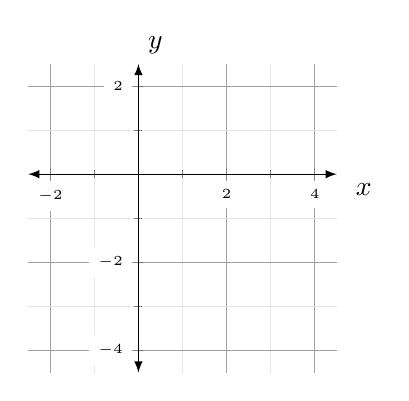
\begin{tikzpicture}[>=latex]
			\begin{axis}[
					    width =5.5cm,
				               height=5.5cm,
					    xmin=-2,xmax=4,
					    ymin=-4,ymax=2,
					    grid=both,
					    grid style={line width=.15pt, draw=gray!20},
					    major grid style={line width=.3pt,draw=gray!75},
					    axis lines=middle,
					    minor tick num=1,
					    enlargelimits={abs=0.5},
					    axis line style={latex-latex},
					    ticklabel style={font=\tiny,fill=white},
					    xlabel={\,\,$x$},
					    ylabel={$y$},
					    xlabel style={below right},
					    ylabel style={above right},
					]
			\end{axis}
			%\draw[color=blue,thick] plot (\x,\x*\x);
	\end{tikzpicture}
\end{minipage}
\begin{minipage}[t]{0.2\linewidth}
	\large
	\vspace{-4.5cm}
	 \begin{tikzpicture}
	 	%%  T-Chart  %%%%%%%%
		\draw (6,5) --(6,0.5);
		\draw (5.5,4.5) node[above]{$x$} (6.5, 4.5) node[above]{$y_1$};
		\draw (5, 4.5) -- (7, 4.5);
		\draw (5.5, 4) node{$1$};
		\draw (5.5, 3.25) node{$2$};
		\draw (5.5, 2.5) node{$3$};
		\draw (5.5, 1.75) node{$4$};
		\draw (5.5, 1) node{$5$};
		%%%%%%%%%%%%%%%
	\end{tikzpicture}
	\normalsize
\end{minipage}
\vfill

%%%%%%%%%%%%%%%%%%%%%%%%%%%%%%%%%%%%%
%%%%%%%%%%%%%%%%%%%%%%%%%%%%%%%%%%%%%
 \newpage
%%%%%%%%%%%%%%%%%%%%%%%%%%%%%%%%%%%%%
%%%%%%%%%%%%%%%%%%%%%%%%%%%%%%%%%%%%%

\begin{center}
	\begin{tabular}{|l|l|}
		\hline
		\multicolumn{2}{|l|}{}\\
		\multicolumn{2}{|c|}{\large\textbf{Translations of Quadratic Functions} \normalsize}\\
		\hline
		&\\
		\multicolumn{1}{|c|}{\textbf{Horizontal Translation}}&\multicolumn{1}{c|}{\textbf{Vertical Translations}}\\	
		&\\
		\hline
		&\\
		\multicolumn{1}{|c|}{\textbf{Horizontal Shift of $|h|$ Units}}&\multicolumn{1}{c|}{\textbf{Vertical Shift of $|k|$ Units}}\\
		\begin{minipage}[t]{0.25\linewidth}
			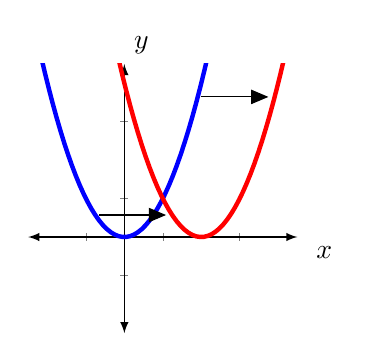
\begin{tikzpicture}[>=triangle 45,]
				\begin{axis}[
						    width = 5cm,
					               height = 5cm,
						    xmin=-2,xmax=4,
						    ymin=-2,ymax=4,
						    grid=none,
						    grid style={line width=.15pt, draw=gray!20},
						    major grid style={line width=.3pt,draw=gray!75},
						    axis lines=middle,
						    minor tick num=1,
						    enlargelimits={abs=0.5},
						    axis line style={latex-latex},
						    ticklabel style={font=\tiny,fill=white},
						    ticks=none,
						    xlabel={\,\,$x$},
						    ylabel={$y$},
						    xlabel style={below right},
						    ylabel style={above right},
						]
						\addplot+[<->, blue, ultra thick,samples=100, mark=none] {x^2};
						\addplot+[<->, red, ultra thick,samples=100,  mark=none] {(x-2)^2};
				\end{axis}
				\draw[->] (0.9,1.5) -- (1.75,1.5);
				\draw[->] (2.2,3) -- (3.05,3);
			\end{tikzpicture}
		\end{minipage}
		\begin{minipage}[t]{0.2\linewidth}
		\vspace{-3.5cm}
		\[f(x)=x^2\]\\
		\vspace{-0.5cm}
		\[f(x\color{red}-h\color{black})=(x\color{red}-h\color{black})^2\]
		Moves left for\\
		$h<0$\\
		Moves right for\\
		$h>0$\\
		\end{minipage}
		&
		\begin{minipage}[t]{0.25\linewidth}
			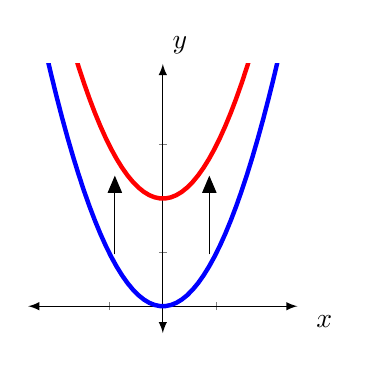
\begin{tikzpicture}[>=triangle 45,]
				\begin{axis}[
						    width = 5cm,
					               height = 5cm,
						    xmin=-2,xmax=2,
						    ymin=0,ymax=4,
						    grid=none,
						    grid style={line width=.15pt, draw=gray!20},
						    major grid style={line width=.3pt,draw=gray!75},
						    axis lines=middle,
						    minor tick num=1,
						    enlargelimits={abs=0.5},
						    axis line style={latex-latex},
						    ticklabel style={font=\tiny,fill=white},
						    ticks=none,
						    xlabel={\,\,$x$},
						    ylabel={$y$},
						    xlabel style={below right},
						    ylabel style={above right},
						]
						\addplot+[<->, blue,samples=100, ultra thick, mark=none] {x^2};
						\addplot+[<->, red,samples=100, ultra thick, mark=none] {x^2+2};
				\end{axis}
				\draw[->] (1.1,1) -- (1.1,2);
				\draw[->] (2.3,1) -- (2.3,2);
			\end{tikzpicture}
		\end{minipage}
		\begin{minipage}[t]{0.2\linewidth}
			\vspace{-3.5cm}
			\[f(x)=x^2\]\\
			\vspace{-0.5cm}
			\[f(x)\color{blue}+k\color{black}=x^2\color{blue}+k\color{black}\]
			Moves up for\\
			$k>0$\\
			Moves down for\\
			$k<0$\\
		\end{minipage}
		\\
		\hline
	\end{tabular}
\end{center}

\begin{example}
Using the graph of $f(x)=x^2$ as a guide, describe the transformations, and then graph each function.
\end{example}

\begin{minipage}[t]{0.45\linewidth}
 (a) \,\, $f(x)=(x+3)^2+1$\\
\end{minipage}
\hfill
\begin{minipage}[t]{0.45\linewidth}
 (b) \,\, $f(x)=(x-2)^2-1$\\
\end{minipage}

\vspace{-0.5cm}

 \begin{minipage}[t]{0.45\linewidth}
	 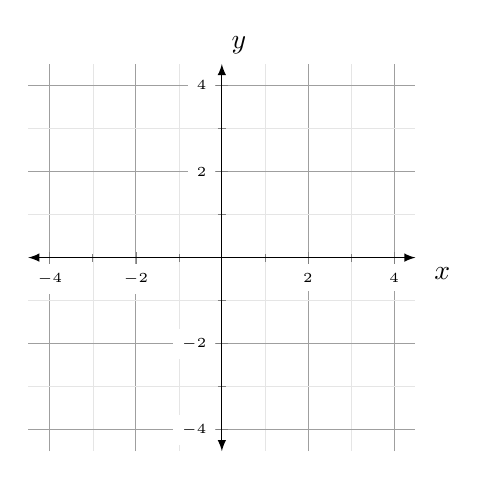
\begin{tikzpicture}[>=latex]
			\begin{axis}[
					    width =6.5cm,
				               height=6.5cm,
					    xmin=-4,xmax=4,
					    ymin=-4,ymax=4,
					    grid=both,
					    grid style={line width=.15pt, draw=gray!20},
					    major grid style={line width=.3pt,draw=gray!75},
					    axis lines=middle,
					    minor tick num=1,
					    enlargelimits={abs=0.5},
					    axis line style={latex-latex},
					    ticklabel style={font=\tiny,fill=white},
					    xlabel={\,\,$x$},
					    ylabel={$y$},
					    xlabel style={below right},
					    ylabel style={above right},
					]
			\end{axis}
	\end{tikzpicture}
\end{minipage}
\hfill
 \begin{minipage}[t]{0.45\linewidth}
	 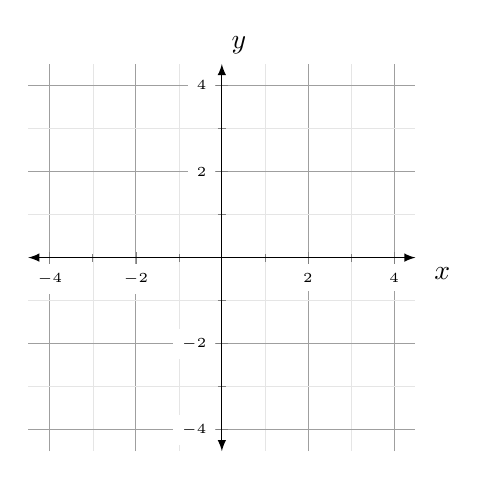
\begin{tikzpicture}[>=latex]
			\begin{axis}[
					    width =6.5cm,
				               height=6.5cm,
					    xmin=-4,xmax=4,
					    ymin=-4,ymax=4,
					    grid=both,
					    grid style={line width=.15pt, draw=gray!20},
					    major grid style={line width=.3pt,draw=gray!75},
					    axis lines=middle,
					    minor tick num=1,
					    enlargelimits={abs=0.5},
					    axis line style={latex-latex},
					    ticklabel style={font=\tiny,fill=white},
					    xlabel={\,\,$x$},
					    ylabel={$y$},
					    xlabel style={below right},
					    ylabel style={above right},
					]
			\end{axis}
	\end{tikzpicture}
\end{minipage}


\begin{youtry}
Using the graph of $f(x)=x^2$ as a guide, describe the transformations, and then graph each function.
\end{youtry}

\begin{minipage}[t]{0.45\linewidth}
 (a) \,\, $f(x)=(x-1)^2+2$\\
\end{minipage}
\hfill
\begin{minipage}[t]{0.45\linewidth}
 (b) \,\, $f(x)=(x+2)^2-3$\\
\end{minipage}

\vspace{-0.5cm}

 \begin{minipage}[t]{0.45\linewidth}
	 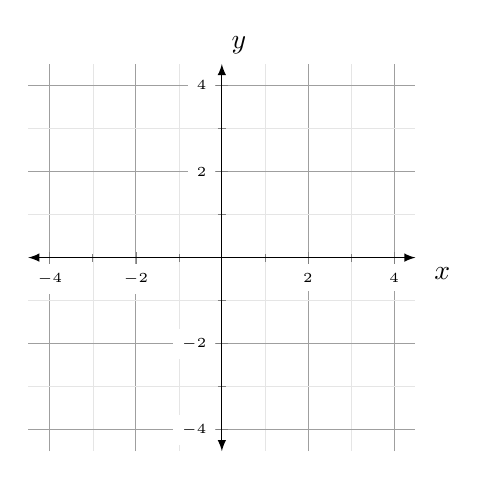
\begin{tikzpicture}[>=latex]
			\begin{axis}[
					    width =6.5cm,
				               height=6.5cm,
					    xmin=-4,xmax=4,
					    ymin=-4,ymax=4,
					    grid=both,
					    grid style={line width=.15pt, draw=gray!20},
					    major grid style={line width=.3pt,draw=gray!75},
					    axis lines=middle,
					    minor tick num=1,
					    enlargelimits={abs=0.5},
					    axis line style={latex-latex},
					    ticklabel style={font=\tiny,fill=white},
					    xlabel={\,\,$x$},
					    ylabel={$y$},
					    xlabel style={below right},
					    ylabel style={above right},
					]
			\end{axis}
	\end{tikzpicture}
\end{minipage}
\hfill
 \begin{minipage}[t]{0.45\linewidth}
	 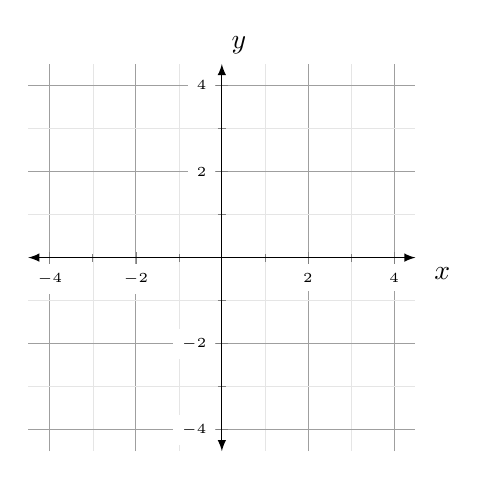
\begin{tikzpicture}[>=latex]
			\begin{axis}[
					    width =6.5cm,
				               height=6.5cm,
					    xmin=-4,xmax=4,
					    ymin=-4,ymax=4,
					    grid=both,
					    grid style={line width=.15pt, draw=gray!20},
					    major grid style={line width=.3pt,draw=gray!75},
					    axis lines=middle,
					    minor tick num=1,
					    enlargelimits={abs=0.5},
					    axis line style={latex-latex},
					    ticklabel style={font=\tiny,fill=white},
					    xlabel={\,\,$x$},
					    ylabel={$y$},
					    xlabel style={below right},
					    ylabel style={above right},
					]
			\end{axis}
	\end{tikzpicture}
\end{minipage}



\vfill
 \noindent\fbox{\large\textbf{5.1  (day 1) Homework}: page 320 \, 2-7, 17-22 all \small }
%%%%%%%%%%%%%%%%%%%%%%%%%%%%%%%%%%%%%
%%%%%%%%%%%%%%%%%%%%%%%%%%%%%%%%%%%%%
 \newpage
%%%%%%%%%%%%%%%%%%%%%%%%%%%%%%%%%%%%%
%%%%%%%%%%%%%%%%%%%%%%%%%%%%%%%%%%%%%

\noindent\Large{\textbf{5.1 (Day 2) Using Transformations to Graph Quadratic Function}}\normalsize\\

\vspace{-0.5cm}

 \hfill \underline{Objective}: Transform quadratic functions. \\

\vspace{-0.5cm}

\begin{center}
	\begin{tabular}{|l|l|}
		\hline
		\multicolumn{2}{|l|}{}\\
		\multicolumn{2}{|c|}{\large\textbf{Reflections of Quadratic Functions} \normalsize}\\
		\hline
		&\\
		\multicolumn{1}{|c|}{\textbf{Reflection Across $\mathbf{y}$-axis}}&\multicolumn{1}{c|}{\textbf{Reflection Across $x$-axis}}\\
		\begin{minipage}[t]{0.25\linewidth}
			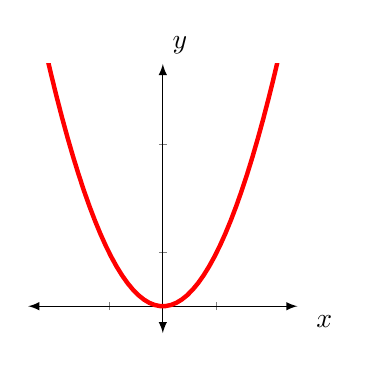
\begin{tikzpicture}[>=triangle 45,]
				\begin{axis}[
						    width = 5cm,
					               height = 5cm,
						    xmin=-2,xmax=2,
						    ymin=0,ymax=4,
						    grid=none,
						    grid style={line width=.15pt, draw=gray!20},
						    major grid style={line width=.3pt,draw=gray!75},
						    axis lines=middle,
						    minor tick num=1,
						    enlargelimits={abs=0.5},
						    axis line style={latex-latex},
						    ticklabel style={font=\tiny,fill=white},
						    ticks=none,
						    xlabel={\,\,$x$},
						    ylabel={$y$},
						    xlabel style={below right},
						    ylabel style={above right},
						]
						\addplot+[<->, red, ultra thick,samples=100, mark=none] {x^2};
				\end{axis}
			\end{tikzpicture}
		\end{minipage}
		\begin{minipage}[t]{0.2\linewidth}
		\vspace{-3.5cm}
		Input values\\
		change.\\
		\[f(x)=x^2\]\\
		\vspace{-0.5cm}
		\[f(\color{red}-\color{black}x)=(\color{red}-\color{black}x)^2 =x^2\]
		The function\\
		$f(x)=x^2$ is its own\\
		reflection across\\
		the $y$-axis\\
		\end{minipage}
		&
		\begin{minipage}[t]{0.25\linewidth}
			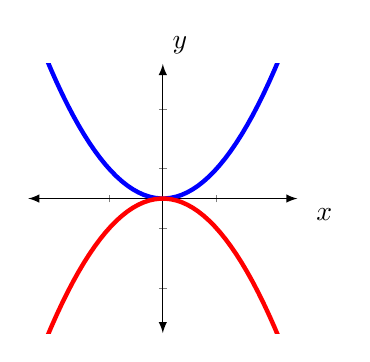
\begin{tikzpicture}[>=triangle 45,]
				\begin{axis}[
						    width = 5cm,
					               height = 5cm,
						    xmin=-2,xmax=2,
						    ymin=-4,ymax=4,
						    grid=none,
						    grid style={line width=.15pt, draw=gray!20},
						    major grid style={line width=.3pt,draw=gray!75},
						    axis lines=middle,
						    minor tick num=1,
						    enlargelimits={abs=0.5},
						    axis line style={latex-latex},
						    ticklabel style={font=\tiny,fill=white},
						    ticks=none,
						    xlabel={\,\,$x$},
						    ylabel={$y$},
						    xlabel style={below right},
						    ylabel style={above right},
						]
						\addplot+[<->, blue,samples=100, ultra thick, mark=none] {x^2};
						\addplot+[<->, red,samples=100, ultra thick, mark=none] {-x^2};
				\end{axis}
			\end{tikzpicture}
		\end{minipage}
		\begin{minipage}[t]{0.2\linewidth}
			\vspace{-3.5cm}
			Input values\\
			change.
			\[f(x)=x^2\]

			\[\color{red}-\color{black}f(x)=\color{red}-\color{black}(x^2)=\color{red}-\color{black}x^2\]
			The function is\\
			flipped across the\\
			$x$-axis.\\
		\end{minipage}
		\\
		\hline
	\end{tabular}
\end{center}

\begin{example}
Using the graph of $f(x)=x^2$ as a guide, describe the transformations, and then graph each function.
\end{example}

\vspace{-0.5cm}

\begin{minipage}[t]{0.45\linewidth}
 (a) \,\, $f(x)=(-(x+1))^2-3$\\
\end{minipage}
\hfill
\begin{minipage}[t]{0.45\linewidth}
 (b) \,\, $f(x)=-(x-1)^2+2$\\
\end{minipage}

\vspace{-0.5cm}

 \begin{minipage}[t]{0.45\linewidth}
	 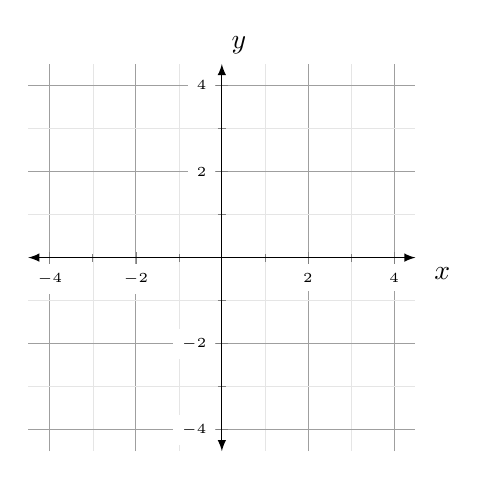
\begin{tikzpicture}[>=latex]
			\begin{axis}[
					    width =6.5cm,
				               height=6.5cm,
					    xmin=-4,xmax=4,
					    ymin=-4,ymax=4,
					    grid=both,
					    grid style={line width=.15pt, draw=gray!20},
					    major grid style={line width=.3pt,draw=gray!75},
					    axis lines=middle,
					    minor tick num=1,
					    enlargelimits={abs=0.5},
					    axis line style={latex-latex},
					    ticklabel style={font=\tiny,fill=white},
					    xlabel={\,\,$x$},
					    ylabel={$y$},
					    xlabel style={below right},
					    ylabel style={above right},
					]
			\end{axis}
	\end{tikzpicture}
\end{minipage}
\hfill
 \begin{minipage}[t]{0.45\linewidth}
	 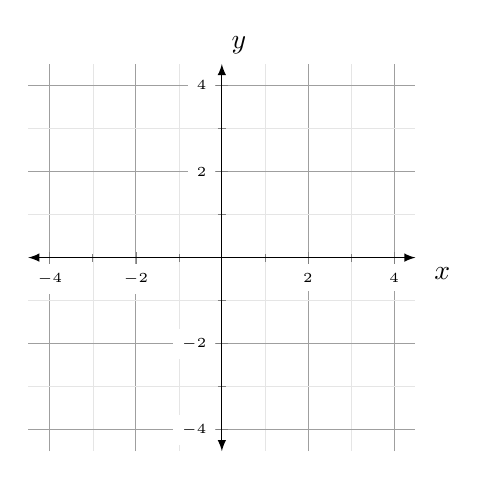
\begin{tikzpicture}[>=latex]
			\begin{axis}[
					    width =6.5cm,
				               height=6.5cm,
					    xmin=-4,xmax=4,
					    ymin=-4,ymax=4,
					    grid=both,
					    grid style={line width=.15pt, draw=gray!20},
					    major grid style={line width=.3pt,draw=gray!75},
					    axis lines=middle,
					    minor tick num=1,
					    enlargelimits={abs=0.5},
					    axis line style={latex-latex},
					    ticklabel style={font=\tiny,fill=white},
					    xlabel={\,\,$x$},
					    ylabel={$y$},
					    xlabel style={below right},
					    ylabel style={above right},
					]
			\end{axis}
	\end{tikzpicture}
\end{minipage}

\begin{youtry}
Using the graph of $f(x)=x^2$ as a guide, describe the transformations, and then graph each function.
\end{youtry}

\vspace{-0.5cm}

\begin{minipage}[t]{0.45\linewidth}
 (a) \,\, $f(x)=-(x+2)^2+1$\\
\end{minipage}
\hfill
\begin{minipage}[t]{0.45\linewidth}
 (b) \,\, $f(x)=(-(x-2))^2-4$\\
\end{minipage}

\vspace{-0.5cm}

 \begin{minipage}[t]{0.45\linewidth}
	 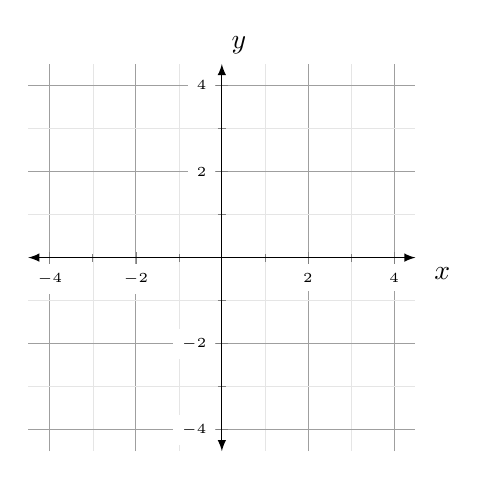
\begin{tikzpicture}[>=latex]
			\begin{axis}[
					    width =6.5cm,
				               height=6.5cm,
					    xmin=-4,xmax=4,
					    ymin=-4,ymax=4,
					    grid=both,
					    grid style={line width=.15pt, draw=gray!20},
					    major grid style={line width=.3pt,draw=gray!75},
					    axis lines=middle,
					    minor tick num=1,
					    enlargelimits={abs=0.5},
					    axis line style={latex-latex},
					    ticklabel style={font=\tiny,fill=white},
					    xlabel={\,\,$x$},
					    ylabel={$y$},
					    xlabel style={below right},
					    ylabel style={above right},
					]
			\end{axis}
	\end{tikzpicture}
\end{minipage}
\hfill
 \begin{minipage}[t]{0.45\linewidth}
	 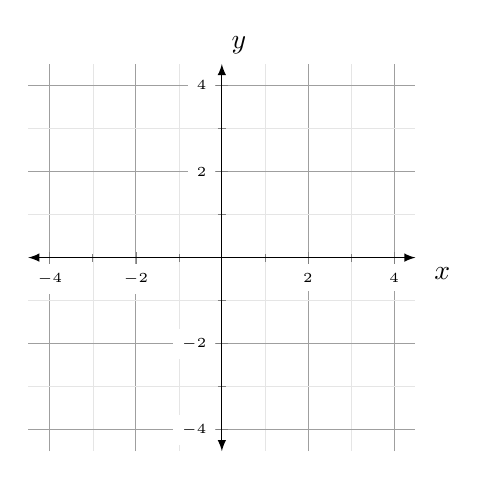
\begin{tikzpicture}[>=latex]
			\begin{axis}[
					    width =6.5cm,
				               height=6.5cm,
					    xmin=-4,xmax=4,
					    ymin=-4,ymax=4,
					    grid=both,
					    grid style={line width=.15pt, draw=gray!20},
					    major grid style={line width=.3pt,draw=gray!75},
					    axis lines=middle,
					    minor tick num=1,
					    enlargelimits={abs=0.5},
					    axis line style={latex-latex},
					    ticklabel style={font=\tiny,fill=white},
					    xlabel={\,\,$x$},
					    ylabel={$y$},
					    xlabel style={below right},
					    ylabel style={above right},
					]
			\end{axis}
	\end{tikzpicture}
\end{minipage}

%%%%%%%%%%%%%%%%%%%%%%%%%%%%%%%%%%%%%
%%%%%%%%%%%%%%%%%%%%%%%%%%%%%%%%%%%%%
 \newpage
%%%%%%%%%%%%%%%%%%%%%%%%%%%%%%%%%%%%%
%%%%%%%%%%%%%%%%%%%%%%%%%%%%%%%%%%%%%

\begin{center}
	\begin{tabular}{|l|l|}
		\hline
		\multicolumn{2}{|l|}{}\\
		\multicolumn{2}{|c|}{\large\textbf{Stretches and Compressions of Quadratic Functions} \normalsize}\\
		\hline
		&\\
		\multicolumn{1}{|c|}{\textbf{Horizontal Stretch/Compression by a}}&\multicolumn{1}{c|}{\textbf{Vertical Stretch/Compression by a}}\\
		\multicolumn{1}{|c|}{\textbf{Factor of $|b|$}}&\multicolumn{1}{c|}{\textbf{Factor of $|a|$}}\\
		\begin{minipage}[t]{0.25\linewidth}
			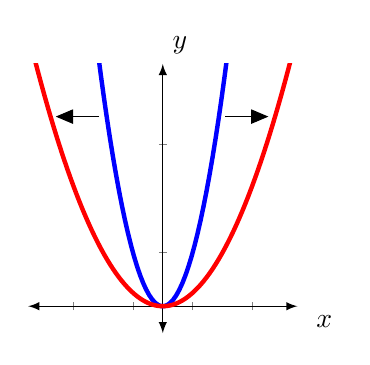
\begin{tikzpicture}[>=triangle 45,]
				\begin{axis}[
						    width = 5cm,
					               height = 5cm,
						    xmin=-4,xmax=4,
						    ymin=0,ymax=4,
						    grid=none,
						    grid style={line width=.15pt, draw=gray!20},
						    major grid style={line width=.3pt,draw=gray!75},
						    axis lines=middle,
						    minor tick num=1,
						    enlargelimits={abs=0.5},
						    axis line style={latex-latex},
						    ticklabel style={font=\tiny,fill=white},
						    ticks=none,
						    xlabel={\,\,$x$},
						    ylabel={$y$},
						    xlabel style={below right},
						    ylabel style={above right},
						]
						\addplot+[<->, blue,samples=100, ultra thick, mark=none] {x^2};
						\addplot+[<->, red, ultra thick,samples=100, mark=none] {(x/2)^2};
				\end{axis}
				\draw[->] (0.9,2.75) -- (0.35,2.75);
				\draw[->] (2.5,2.75) -- (3.05,2.75);
			\end{tikzpicture}
		\end{minipage}
		\begin{minipage}[t]{0.2\linewidth}
		\vspace{-3.5cm}
		Input values\\
		change.\\
		\[f(x)=x^2\]\\
		\vspace{-0.5cm}
		\[f\bigg{(}\color{red}\displaystyle\frac{1}{b}\color{black}x\bigg{)}=\bigg{(}\color{red}\displaystyle\frac{1}{b}\color{black}x\bigg{)}^2\]
		\end{minipage}
		&
		\begin{minipage}[t]{0.25\linewidth}
			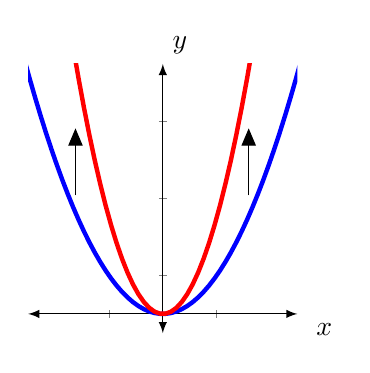
\begin{tikzpicture}[>=triangle 45,]
				\begin{axis}[
						    width = 5cm,
					               height = 5cm,
						    xmin=-2,xmax=2,
						    ymin=0,ymax=6,
						    grid=none,
						    grid style={line width=.15pt, draw=gray!20},
						    major grid style={line width=.3pt,draw=gray!75},
						    axis lines=middle,
						    minor tick num=1,
						    enlargelimits={abs=0.5},
						    axis line style={latex-latex},
						    ticklabel style={font=\tiny,fill=white},
						    ticks=none,
						    xlabel={\,\,$x$},
						    ylabel={$y$},
						    xlabel style={below right},
						    ylabel style={above right},
						]
						\addplot+[<->, blue,samples=100, ultra thick, mark=none] {x^2};
						\addplot+[<->, red,samples=100, ultra thick, mark=none] {2.5*x^2};
				\end{axis}
				\draw[->] (0.6,1.75) -- (0.6,2.6);
				\draw[->] (2.8,1.75) -- (2.8,2.6);
			\end{tikzpicture}
		\end{minipage}
		\begin{minipage}[t]{0.2\linewidth}
			\vspace{-3.5cm}
			Input values\\
			change.
			\[f(x)=x^2\]

			\[\color{red}a\color{black}f(x)=\color{red}a\color{black}(x^2)\]
		\end{minipage}\\
		&\\
		\multicolumn{1}{|c|}{$|b|>1$ stretches away from the $y$-axis} & \multicolumn{1}{|c|}{$|a|>1$ stretches away from the $x$-axis}\\
		&\\
		\multicolumn{1}{|c|}{$0<|b|<1$ compresses toward the $y$-axis} & \multicolumn{1}{|c|}{$0<|a|<1$ compresses toward the $x$-axis}\\
		\hline
	\end{tabular}
\end{center}

\begin{example}
Using the graph of $f(x)=x^2$ as a guide, describe the transformations, and then graph each function.
\end{example}

\vspace{-0.5cm}

\begin{minipage}[t]{0.45\linewidth}
 (a) \,\, $g(x)=-4x^2$\\
\end{minipage}
\hfill
\begin{minipage}[t]{0.45\linewidth}
 (b) \,\, $g(x)=-\bigg{(}\displaystyle\frac{1}{2}x\bigg{)}^2$\\
\end{minipage}

\vspace{-0.5cm}

 \begin{minipage}[t]{0.45\linewidth}
	 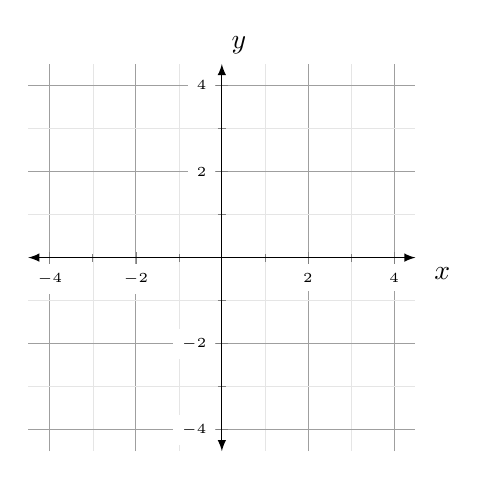
\begin{tikzpicture}[>=latex]
			\begin{axis}[
					    width =6.5cm,
				               height=6.5cm,
					    xmin=-4,xmax=4,
					    ymin=-4,ymax=4,
					    grid=both,
					    grid style={line width=.15pt, draw=gray!20},
					    major grid style={line width=.3pt,draw=gray!75},
					    axis lines=middle,
					    minor tick num=1,
					    enlargelimits={abs=0.5},
					    axis line style={latex-latex},
					    ticklabel style={font=\tiny,fill=white},
					    xlabel={\,\,$x$},
					    ylabel={$y$},
					    xlabel style={below right},
					    ylabel style={above right},
					]
			\end{axis}
	\end{tikzpicture}
\end{minipage}
\hfill
 \begin{minipage}[t]{0.45\linewidth}
	 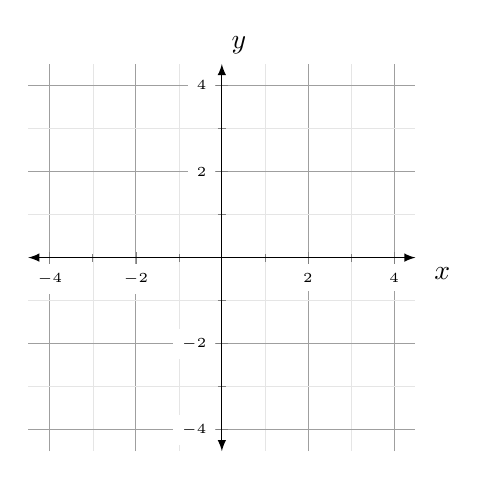
\begin{tikzpicture}[>=latex]
			\begin{axis}[
					    width =6.5cm,
				               height=6.5cm,
					    xmin=-4,xmax=4,
					    ymin=-4,ymax=4,
					    grid=both,
					    grid style={line width=.15pt, draw=gray!20},
					    major grid style={line width=.3pt,draw=gray!75},
					    axis lines=middle,
					    minor tick num=1,
					    enlargelimits={abs=0.5},
					    axis line style={latex-latex},
					    ticklabel style={font=\tiny,fill=white},
					    xlabel={\,\,$x$},
					    ylabel={$y$},
					    xlabel style={below right},
					    ylabel style={above right},
					]
			\end{axis}
	\end{tikzpicture}
\end{minipage}

\begin{youtry}
Using the graph of $f(x)=x^2$ as a guide, describe the transformations, and then graph each function.
\end{youtry}

\vspace{-0.5cm}

\begin{minipage}[t]{0.45\linewidth}
 (a) \,\, $g(x)=(2x)^2$\\
\end{minipage}
\hfill
\begin{minipage}[t]{0.45\linewidth}
 (b) \,\, $h(x)=\displaystyle-\frac{1}{2}(x-1)^2$\\
\end{minipage}

\vspace{-0.5cm}

 \begin{minipage}[t]{0.45\linewidth}
	 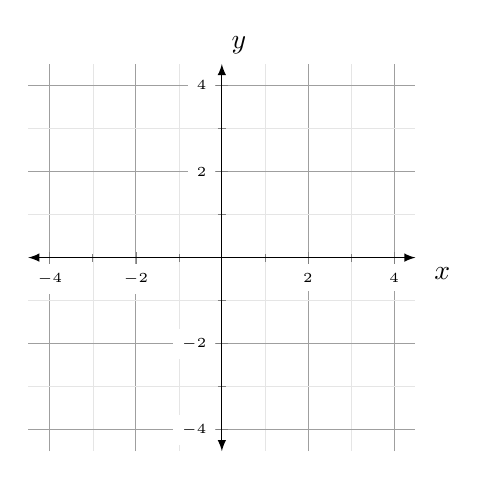
\begin{tikzpicture}[>=latex]
			\begin{axis}[
					    width =6.5cm,
				               height=6.5cm,
					    xmin=-4,xmax=4,
					    ymin=-4,ymax=4,
					    grid=both,
					    grid style={line width=.15pt, draw=gray!20},
					    major grid style={line width=.3pt,draw=gray!75},
					    axis lines=middle,
					    minor tick num=1,
					    enlargelimits={abs=0.5},
					    axis line style={latex-latex},
					    ticklabel style={font=\tiny,fill=white},
					    xlabel={\,\,$x$},
					    ylabel={$y$},
					    xlabel style={below right},
					    ylabel style={above right},
					]
			\end{axis}
	\end{tikzpicture}
\end{minipage}
\hfill
 \begin{minipage}[t]{0.45\linewidth}
	 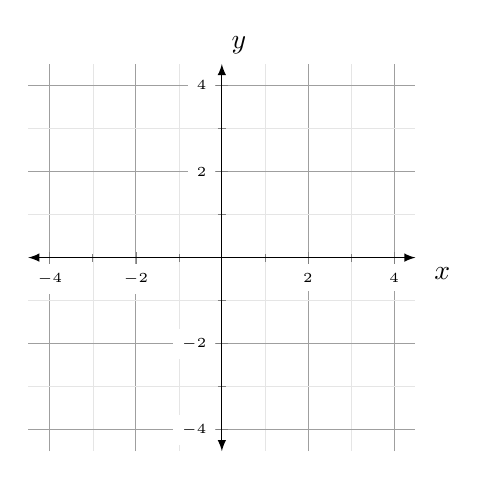
\begin{tikzpicture}[>=latex]
			\begin{axis}[
					    width =6.5cm,
				               height=6.5cm,
					    xmin=-4,xmax=4,
					    ymin=-4,ymax=4,
					    grid=both,
					    grid style={line width=.15pt, draw=gray!20},
					    major grid style={line width=.3pt,draw=gray!75},
					    axis lines=middle,
					    minor tick num=1,
					    enlargelimits={abs=0.5},
					    axis line style={latex-latex},
					    ticklabel style={font=\tiny,fill=white},
					    xlabel={\,\,$x$},
					    ylabel={$y$},
					    xlabel style={below right},
					    ylabel style={above right},
					]
			\end{axis}
	\end{tikzpicture}
\end{minipage}


\vfill
 \noindent\fbox{\large\textbf{5.1  (day 2) Homework}: page 320\, 23-28 all, 33, 35, 37, Adv. 29, 30, 39-41 all  \normalsize }

%%%%%%%%%%%%%%%%%%%%%%%%%%%%%%%%%%%%%
%%%%%%%%%%%%%%%%%%%%%%%%%%%%%%%%%%%%%
 \newpage
%%%%%%%%%%%%%%%%%%%%%%%%%%%%%%%%%%%%%
%%%%%%%%%%%%%%%%%%%%%%%%%%%%%%%%%%%%%

%%%%%%%%%%%%%%%%%%%%%%%%%%%%%%%
%%%%%%%%%%%%%%%%%%%%%%%%%%%%%%%
%%%%%%   Section 5.2   %%%%%%%%
%%%%%%%%%%%%%%%%%%%%%%%%%%%%%%%
%%%%%%%%%%%%%%%%%%%%%%%%%%%%%%%
 \section{ Properties of Quadratics in Standard Form  }
 \setcounter{example}{0}
 \setcounter{definition}{0}
\vspace{-0.5cm}
 \hfill \underline{Objective}: Define, identify, and graph quadratic functions. Use the vertex and standard form to graph quadratics.\\
 %%%%%%%%%%%%%%%%%%%%%%%%%%%%%%%%
 %%%%%%%%%%%%%%%%%%%%%%%%%%%%%%%%

\begin{definition}
If a parabola opens upward, it has a lowest point. If a parabola opens downward, it has a highest point. This lowest or highest point is called the \textbf{vertex} of the parabola.
\end{definition}

\vspace{-0.5cm}

\begin{center}
\textbf{Vertex Form of a Quadratic Function}\\

\vspace{0.15cm}

\large\fbox{$f(x) = \color{red}\mathbf{a}\color{black}\big{(}x-\color{blue}\mathbf{h}\color{black}\big{)}^2+\color{green}\mathbf{k}\color{black}$}\normalsize\\

\hspace{3cm}
\begin{minipage}[t]{0.3\linewidth}
\color{red}
\textbf{$\mathbf{a}$ indicates a reflection\\
across the $\mathbf{x}$-axis and/or\\
a vertical stretch or\\ compression.
}
\color{black}
\end{minipage}
\begin{minipage}[t]{0.2\linewidth}
\color{blue}
\textbf{
\noindent$\mathbf{h}$ indicates\\ a horizontal \\ translation.
}
\color{black}
\end{minipage}
\begin{minipage}[t]{0.3\linewidth}
\color{green}
\textbf{
$\mathbf{k}$ indicates a \\ vertical translation.
}
\color{black}
\end{minipage}
\end{center}

\noindent In \textbf{vertex form} of a parabola the vertex can be read as $\color{blue}\mathbf{h}\color{black}$ horizontal units and $\mathbf{\color{green}k\color{black}}$ vertical units from the origin, the vertex of the parabola is at $\mathbf{(\color{blue}h\color{black},\color{green}k\color{black})}$.

 \begin{example}
Use the description to write the equation in vertex form.
 \end{example}
 
 \vspace{-0.5cm}
 
\begin{minipage}[t]{0.45\linewidth}
	(a) The parent function $f(x)=x^2$ is vertically compressed by a factor of $\frac{1}{3}$ and translated 2 units right and $4$ units down to create $g$.
\end{minipage}
\hfill
\begin{minipage}[t]{0.45\linewidth}
	(b) The parent function $f(x)=x^2$ is reflected across the $x$-axis and translated $5$ units left and $1$ unit up to create $g$.
\end{minipage}
 
 
 \vspace{1.5cm}
 
\begin{example}
Graph the equations found in the previous examples.
\end{example}
 
 \vspace{-0.5cm}
 
  \begin{minipage}[t]{0.45\linewidth}
	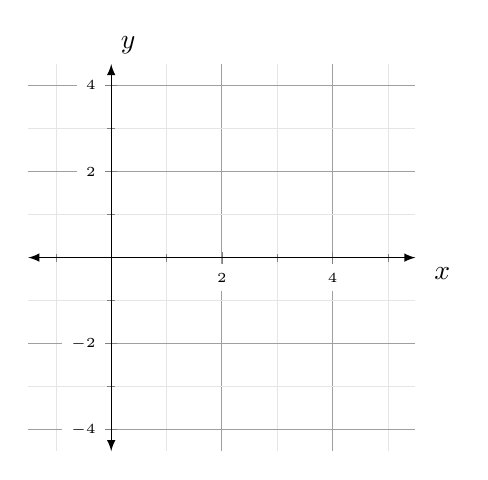
\begin{tikzpicture}[>=latex]
			\begin{axis}[
					    width =6.5cm,
				               height=6.5cm,
					    xmin=-1,xmax=5,
					    ymin=-4,ymax=4,
					    grid=both,
					    grid style={line width=.15pt, draw=gray!20},
					    major grid style={line width=.3pt,draw=gray!75},
					    axis lines=middle,
					    minor tick num=1,
					    enlargelimits={abs=0.5},
					    axis line style={latex-latex},
					    ticklabel style={font=\tiny,fill=white},
					    xlabel={\,\,$x$},
					    ylabel={$y$},
					    xlabel style={below right},
					    ylabel style={above right},
					]
			\end{axis}
	\end{tikzpicture}
\end{minipage}
\hfill
 \begin{minipage}[t]{0.45\linewidth}
	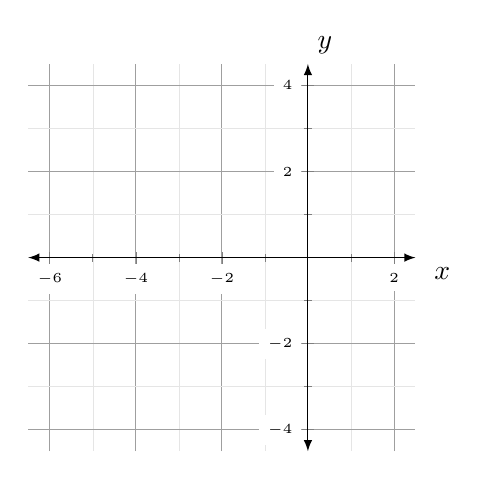
\begin{tikzpicture}[>=latex]
			\begin{axis}[
					    width =6.5cm,
				               height=6.5cm,
					    xmin=-6,xmax=2,
					    ymin=-4,ymax=4,
					    grid=both,
					    grid style={line width=.15pt, draw=gray!20},
					    major grid style={line width=.3pt,draw=gray!75},
					    axis lines=middle,
					    minor tick num=1,
					    enlargelimits={abs=0.5},
					    axis line style={latex-latex},
					    ticklabel style={font=\tiny,fill=white},
					    xlabel={\,\,$x$},
					    ylabel={$y$},
					    xlabel style={below right},
					    ylabel style={above right},
					]
			\end{axis}
	\end{tikzpicture}
\end{minipage}
 
 \vspace{0.5cm}
 
 \begin{definition}
 The \textbf{axis of symmetry} is the line through the vertex of a parabola that divides the parabola into two congruent halves.
 \end{definition}
 
 \vspace{-0.5cm}
 
 \begin{center}
 \begin{tabular}[t]{|l|l|l|}
 \hline
 \multicolumn{1}{|c|}{\textbf{Words}} &  \multicolumn{1}{c|}{\textbf{Algebra}} &  \multicolumn{1}{c|}{\textbf{Graph}}  \\
 \hline
 &&\\
 \begin{minipage}{0.3\linewidth}
 \vspace{-2cm}
 The axis of symmetry is a vertical line through the vertex of the function's  graph.\\
\end{minipage}
  &
\begin{minipage}{0.3\linewidth}
 \vspace{-2cm}
The quadratic function $f(x)=a(x-h)^2+k$ has the axis of symmetry $x=h$. \\
\end{minipage}
  &
\begin{minipage}{0.3\linewidth}
\vspace{-0.25cm}
\begin{center}
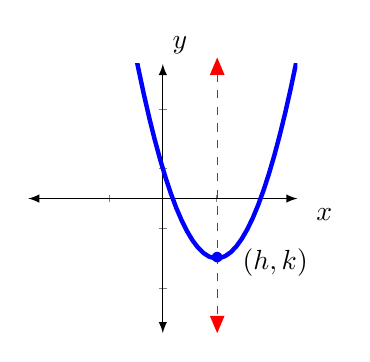
\begin{tikzpicture}[>=triangle 45,]
				\begin{axis}[
						    width = 5cm,
					               height = 5cm,
						    xmin=-2,xmax=2,
						    ymin=-4,ymax=4,
						    grid=none,
						    grid style={line width=.15pt, draw=gray!20},
						    major grid style={line width=.3pt,draw=gray!75},
						    axis lines=middle,
						    minor tick num=1,
						    enlargelimits={abs=0.5},
						    axis line style={latex-latex},
						    ticklabel style={font=\tiny,fill=white},
						    ticks=none,
						    xlabel={\,\,$x$},
						    ylabel={$y$},
						    xlabel style={below right},
						    ylabel style={above right},
						]
						\addplot+[<->, blue ,samples=100, ultra thick, mark=none] {3*(x-1)^2-2};
				\end{axis}
				\draw[<->,dashed, red] (2.4,0) -- (2.4,3.5);
				\draw (2.6,0.9) node[right]{$(h,k)$};
				\draw[blue] (2.4,0.95) node{$\bullet$};
 \end{tikzpicture}
 \end{center}
 \end{minipage}\\
 &&\\
 \hline
 \end{tabular}
 \end{center}



%%%%%%%%%%%%%%%%%%%%%%%%%%%%%%%%%%%%%
%%%%%%%%%%%%%%%%%%%%%%%%%%%%%%%%%%%%%
 \newpage
%%%%%%%%%%%%%%%%%%%%%%%%%%%%%%%%%%%%%
%%%%%%%%%%%%%%%%%%%%%%%%%%%%%%%%%%%%%

\noindent \large\textbf{Properties of a Parabola}\normalsize\\

\vspace{-0.5cm}

\noindent For $f(x) = ax^2+bx+c$, where $a$, $b$, and $c$ are real numbers and $a\neq 0$, the parabola has these properties:\\

\vspace{-0.5cm}

\noindent Parabola \textbf{\color{red}opens\color{black}} upward if $\mathbf{a>0}$ and downward if $\mathbf{a<0}$.\\
The \textbf{\color{red}axis of symmetry\color{black}} is the vertical line $\mathbf{x=\displaystyle-\frac{b}{2a}}$.\\
The \textbf{\color{red}vertex\color{black}} is the point $\mathbf{\bigg{(}\displaystyle-\frac{b}{2a}, f\bigg{(}-\frac{b}{2a}\bigg{)}\bigg{)}.}$\\
The \textbf{\color{red}y-intercept\color{black}} is $\mathbf{c}$.

\begin{example}
For each function \textbf{(a)} determine whether the graph opens upward or downward. \textbf{(b)} Find the axis of symmetry. \textbf{(c)} Find the vertex. \textbf{(d)} Find the $y$-intercept. \textbf{(e)} Graph the function.
\end{example}

\vspace{-0.25cm}

\begin{minipage}[t]{0.45\linewidth}
$f(x)=x^2-4x+6$\\

(a) Opens: \hfill (c) Vertex: \hfill\,\\

(b) Axis:\hfill (d) $y$-int: \hfill\,\\

(e) \quad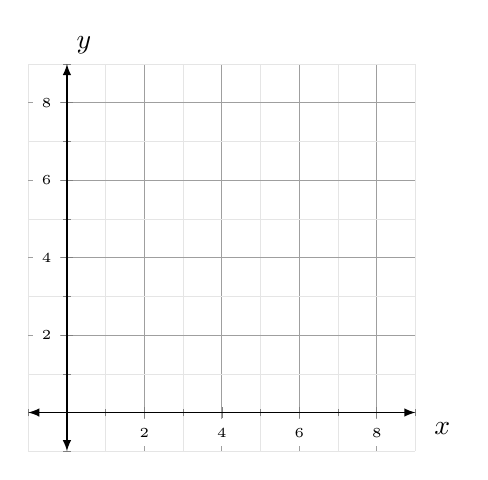
\begin{tikzpicture}[>=latex]
			\begin{axis}[
					    width =6.5cm,
				               height=6.5cm,
					    xmin=0,xmax=8,
					    ymin=0,ymax=8,
					    grid=both,
					    grid style={line width=.15pt, draw=gray!20},
					    major grid style={line width=.3pt,draw=gray!75},
					    axis lines=middle,
					    minor tick num=1,
					    enlargelimits={abs=1},
					    axis line style={latex-latex},
					    ticklabel style={font=\tiny,fill=white},
					    xlabel={\,\,$x$},
					    ylabel={$y$},
					    xlabel style={below right},
					    ylabel style={above right},
					]
			\end{axis}
	\end{tikzpicture}
\end{minipage}
\hfill
\begin{minipage}[t]{0.45\linewidth}
$g(x)=-4x^2-12x-3$\\

(a) Opens: \hfill (c) Vertex: \hfill\,\\

(b) Axis:\hfill (d) $y$-int: \hfill\,\\

(e) \quad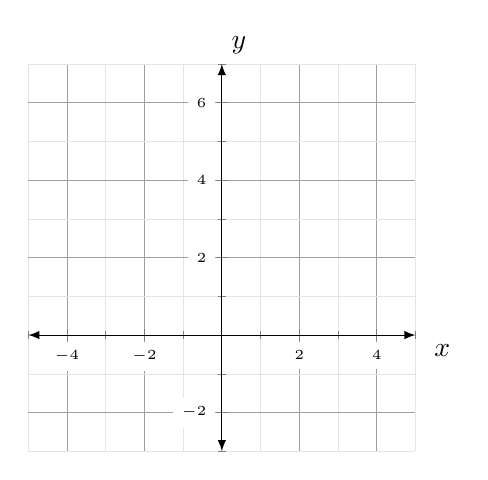
\begin{tikzpicture}[>=latex]
			\begin{axis}[
					    width =6.5cm,
				               height=6.5cm,
					    xmin=-4,xmax=4,
					    ymin=-2,ymax=6,
					    grid=both,
					    grid style={line width=.15pt, draw=gray!20},
					    major grid style={line width=.3pt,draw=gray!75},
					    axis lines=middle,
					    minor tick num=1,
					    enlargelimits={abs=1},
					    axis line style={latex-latex},
					    ticklabel style={font=\tiny,fill=white},
					    xlabel={\,\,$x$},
					    ylabel={$y$},
					    xlabel style={below right},
					    ylabel style={above right},
					]
			\end{axis}
	\end{tikzpicture}
\end{minipage}

\begin{minipage}[t]{0.45\linewidth}
$h(x)=-2x^2-4x$\\

(a) Opens: \hfill (c) Vertex: \hfill\,\\

(b) Axis:\hfill (d) $y$-int: \hfill\,\\

(e) \quad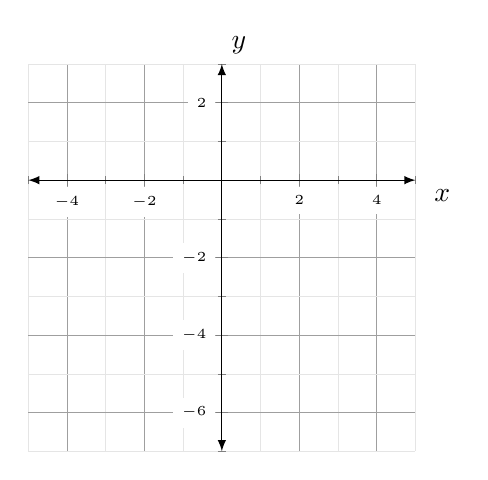
\begin{tikzpicture}[>=latex]
			\begin{axis}[
					    width =6.5cm,
				               height=6.5cm,
					    xmin=-4,xmax=4,
					    ymin=-6,ymax=2,
					    grid=both,
					    grid style={line width=.15pt, draw=gray!20},
					    major grid style={line width=.3pt,draw=gray!75},
					    axis lines=middle,
					    minor tick num=1,
					    enlargelimits={abs=1},
					    axis line style={latex-latex},
					    ticklabel style={font=\tiny,fill=white},
					    xlabel={\,\,$x$},
					    ylabel={$y$},
					    xlabel style={below right},
					    ylabel style={above right},
					]
			\end{axis}
	\end{tikzpicture}
\end{minipage}
\hfill
\begin{minipage}[t]{0.45\linewidth}
$p(x)=x^2+3x-1$\\

(a) Opens: \hfill (c) Vertex: \hfill\,\\

(b) Axis:\hfill (d) $y$-int: \hfill\,\\

(e)\quad 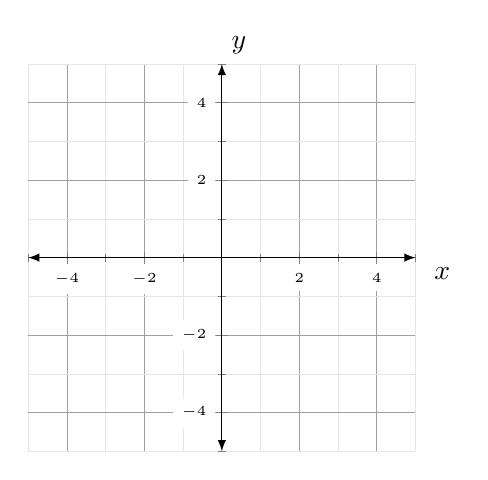
\begin{tikzpicture}[>=latex]
			\begin{axis}[
					    width =6.5cm,
				               height=6.5cm,
					    xmin=-4,xmax=4,
					    ymin=-4,ymax=4,
					    grid=both,
					    grid style={line width=.15pt, draw=gray!20},
					    major grid style={line width=.3pt,draw=gray!75},
					    axis lines=middle,
					    minor tick num=1,
					    enlargelimits={abs=1},
					    axis line style={latex-latex},
					    ticklabel style={font=\tiny,fill=white},
					    xlabel={\,\,$x$},
					    ylabel={$y$},
					    xlabel style={below right},
					    ylabel style={above right},
					]
			\end{axis}
	\end{tikzpicture}
\end{minipage}

\vfill
 \noindent\fbox{\large\textbf{5.2 (day 1) Homework}: page 328\, 2-7, 13, 15, 17 Adv. 39, 42, 43 \small }
%%%%%%%%%%%%%%%%%%%%%%%%%%%%%%%%%%%%%
%%%%%%%%%%%%%%%%%%%%%%%%%%%%%%%%%%%%%
 \newpage
%%%%%%%%%%%%%%%%%%%%%%%%%%%%%%%%%%%%%
%%%%%%%%%%%%%%%%%%%%%%%%%%%%%%%%%%%%%

\noindent\Large{\textbf{5.2 (Day 2) Properties of Quadratic Functions in Standard Form}}\normalsize\\

\vspace{-0.5cm}

 \hfill \underline{Objective}: Identify and use maximums and minimums of quadratic functions to solve problems. \\

\vspace{-0.25cm}

\begin{youtry}
For each function \textbf{(a)} determine whether the graph opens upward or downward. \textbf{(b)} Find the axis of symmetry. \textbf{(c)} Find the vertex. \textbf{(d)} Find the $y$-intercept. \textbf{(e)} Graph the function.
\end{youtry}

\vspace{-0.5cm}

\begin{minipage}[t]{0.45\linewidth}
$f(x)=x^2-4x+5$\\

(a) Opens: \hfill (c) Vertex: \hfill\,\\

(b) Axis:\hfill (d) $y$-int: \hfill\,\\

(e) \quad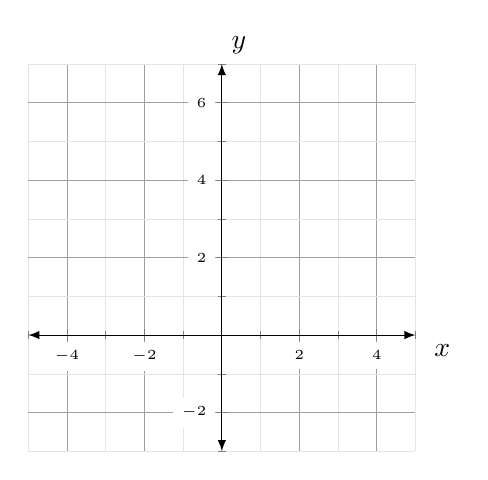
\begin{tikzpicture}[>=latex]
			\begin{axis}[
					    width =6.5cm,
				               height=6.5cm,
					    xmin=-4,xmax=4,
					    ymin=-2,ymax=6,
					    grid=both,
					    grid style={line width=.15pt, draw=gray!20},
					    major grid style={line width=.3pt,draw=gray!75},
					    axis lines=middle,
					    minor tick num=1,
					    enlargelimits={abs=1},
					    axis line style={latex-latex},
					    ticklabel style={font=\tiny,fill=white},
					    xlabel={\,\,$x$},
					    ylabel={$y$},
					    xlabel style={below right},
					    ylabel style={above right},
					]
			\end{axis}
	\end{tikzpicture}
\end{minipage}
\hfill
\begin{minipage}[t]{0.45\linewidth}
$g(x)=x^2+6x+6$\\

(a) Opens: \hfill (c) Vertex: \hfill\,\\

(b) Axis:\hfill (d) $y$-int: \hfill\,\\

(e)\quad 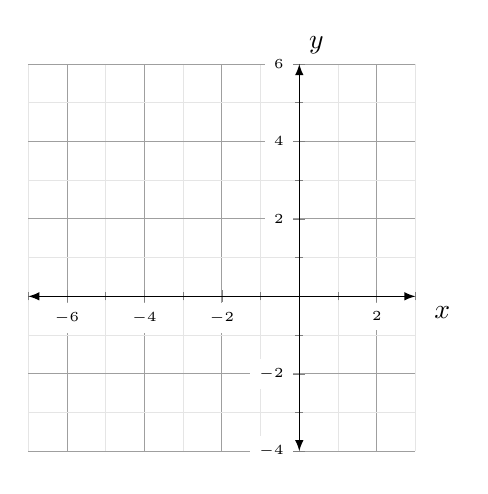
\begin{tikzpicture}[>=latex]
			\begin{axis}[
					    width =6.5cm,
				               height=6.5cm,
					    xmin=-6,xmax=2,
					    ymin=-3,ymax=5,
					    grid=both,
					    grid style={line width=.15pt, draw=gray!20},
					    major grid style={line width=.3pt,draw=gray!75},
					    axis lines=middle,
					    minor tick num=1,
					    enlargelimits={abs=1},
					    axis line style={latex-latex},
					    ticklabel style={font=\tiny,fill=white},
					    xlabel={\,\,$x$},
					    ylabel={$y$},
					    xlabel style={below right},
					    ylabel style={above right},
					]
			\end{axis}
	\end{tikzpicture}
\end{minipage}

\vspace{-0.75cm}

\begin{center}
	\begin{tabular}{|l|l|}
		\hline
		\multicolumn{2}{|l|}{}\\
		\multicolumn{2}{|c|}{\large\textbf{Minimum and Maximum Values} \normalsize}\\
		\hline
		&\\
		\multicolumn{1}{|c|}{\textbf{Opens Upward}}&\multicolumn{1}{c|}{\textbf{Opens Downward}}\\
		\hline
		&\\
		When a parabola opens upward, the $y$-value of the & When a parabola opens downward, the $y$-value of the\\
		 vertex is the \textbf{minimum value}. &   vertex is the \textbf{maximum value}. \\
		&\\
		\begin{minipage}[t]{0.21\linewidth}
		\vspace{-3cm}
		\[D:\bigg{\{}x|x\in\mathbb{R}\bigg{\}}\]
		\[R:\bigg{\{}y|y\geq k\bigg{\}}\]
		\end{minipage}
		\begin{minipage}[t]{0.24\linewidth}
			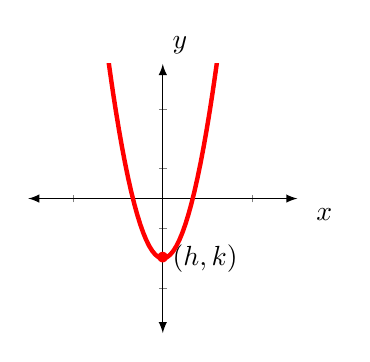
\begin{tikzpicture}[>=triangle 45,]
				\begin{axis}[
						    width = 5cm,
					               height = 5cm,
						    xmin=-4,xmax=4,
						    ymin=-4,ymax=4,
						    grid=none,
						    grid style={line width=.15pt, draw=gray!20},
						    major grid style={line width=.3pt,draw=gray!75},
						    axis lines=middle,
						    minor tick num=1,
						    enlargelimits={abs=0.5},
						    axis line style={latex-latex},
						    ticklabel style={font=\tiny,fill=white},
						    ticks=none,
						    xlabel={\,\,$x$},
						    ylabel={$y$},
						    xlabel style={below right},
						    ylabel style={above right},
						]
						\addplot+[<->, red, ultra thick,samples=100, mark=none] {2*x^2-2};
						\draw (0,-2) node[right]{$(h,k)$};
						\draw[red] (0,-2) node{$\bullet$};
				\end{axis}
			\end{tikzpicture}
		\end{minipage}
		&
		\begin{minipage}[t]{0.21\linewidth}
		\vspace{-3cm}
		\[D:\bigg{\{}x|x\in\mathbb{R}\bigg{\}}\]
		\[R:\bigg{\{}y|y\leq k\bigg{\}}\]
		\end{minipage}
		\begin{minipage}[t]{0.24\linewidth}
			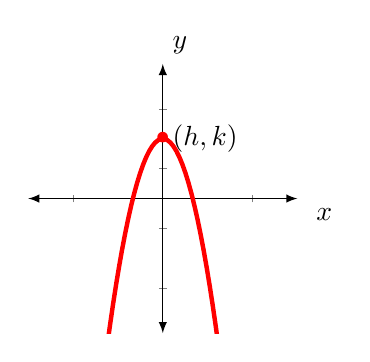
\begin{tikzpicture}[>=triangle 45,]
				\begin{axis}[
						    width = 5cm,
					               height = 5cm,
						    xmin=-4,xmax=4,
						    ymin=-4,ymax=4,
						    grid=none,
						    grid style={line width=.15pt, draw=gray!20},
						    major grid style={line width=.3pt,draw=gray!75},
						    axis lines=middle,
						    minor tick num=1,
						    enlargelimits={abs=0.5},
						    axis line style={latex-latex},
						    ticklabel style={font=\tiny,fill=white},
						    ticks=none,
						    xlabel={\,\,$x$},
						    ylabel={$y$},
						    xlabel style={below right},
						    ylabel style={above right},
						]
						\addplot+[<->, red,samples=100, ultra thick, mark=none] {-2*x^2+2};
						\draw (0,2) node[right]{$(h,k)$};
						\draw[red] (0,2) node{$\bullet$};
				\end{axis}
			\end{tikzpicture}
		\end{minipage}\\
		The domain is all real number, $\mathbb{R}$. The range is all  & The domain is all real numbers, $\mathbb{R}$. The range is all \\
		values greater than or equal  to the minimum.& values less than or equal to the maximum.\\
		& \\
		\hline
	\end{tabular}
\end{center}

\begin{example}
Find the minimum or maximum value of each function. Then state the domain and range of the function.
\end{example}

\vspace{-0.5cm}

\vspace{-0.25cm}

\begin{minipage}[t]{0.45\linewidth}
(a) $f(x)=2x^2-2x+5$\\

\underline{Max/Min}:\\

\underline{Domain}:\\

\underline{Range}:\\
\end{minipage}
\begin{minipage}[t]{0.45\linewidth}
(b) $f(x)=x^2-6x+3$\\

\underline{Max/Min}:\\

\underline{Domain}:\\

\underline{Range}:\\
\end{minipage}


%%%%%%%%%%%%%%%%%%%%%%%%%%%%%%%%%%%%%
%%%%%%%%%%%%%%%%%%%%%%%%%%%%%%%%%%%%%
 \newpage
%%%%%%%%%%%%%%%%%%%%%%%%%%%%%%%%%%%%%
%%%%%%%%%%%%%%%%%%%%%%%%%%%%%%%%%%%%%


\begin{example}
The power $p$ in horsepower (hp) generated by a speedboat engine operating at $r$ revolutions per minute (rpm) can be modeled by
the function $p(r)=-0.0000147r^2+0.18r-251$. What is the maximum power of this engine to the nearest horsepower? At how many 
revolutions per minute must the engine be operating to achieve this power?
\end{example}
\vfill
\begin{example}
The highway mileage $m$ in miles per gallon for a compact car is approximated by $m(s) = -0.025s^2+2.45s-30$, where $s$ is the speed 
in miles per hour. What is the maximum mileage for this compact car to the nearest tenth of a mile per gallon? What speed results in this
 mileage?
\end{example}

\vfill

 \noindent\fbox{\large\textbf{5.2 (day 2) Homework}: page 328\, 8-10 all, 12-30 multiples of 3, Adv. 35, 40 \small }

%%%%%%%%%%%%%%%%%%%%%%%%%%%%%%%%%%%%%
%%%%%%%%%%%%%%%%%%%%%%%%%%%%%%%%%%%%%
 \newpage
%%%%%%%%%%%%%%%%%%%%%%%%%%%%%%%%%%%%%
%%%%%%%%%%%%%%%%%%%%%%%%%%%%%%%%%%%%%


%%%%%%%%%%%%%%%%%%%%%%%%%%%%%%%
%%%%%%%%%%%%%%%%%%%%%%%%%%%%%%%
%%%%%%   Section 5.3   %%%%%%%%
%%%%%%%%%%%%%%%%%%%%%%%%%%%%%%%
%%%%%%%%%%%%%%%%%%%%%%%%%%%%%%%
 \section{ Solving Quadratic Equations by Graphing and Factoring  }
 \setcounter{example}{0}
 \setcounter{definition}{0}
 \setcounter{youtry}{0}
 \hfill \small \underline{Objective}: Solve quadratic equations by graphing and factoring.\\ \hfill \indent \hfill Determine a quadratic function from its roots. \normalsize \\
 %%%%%%%%%%%%%%%%%%%%%%%%%%%%%%%%
 %%%%%%%%%%%%%%%%%%%%%%%%%%%%%%%%
 \begin{definition}
A \textbf{zero of a function} is a value of the input $x$ that makes the output $f(x)$ equal zero. The zeros of a function are the $x$-intercepts.
 \end{definition}
 \begin{example}
Find the zeros of the following functions by using a graph and table.
 \end{example}

\begin{minipage}[t]{0.45\linewidth}
(a) $f(x)=x^2+2x-3$
\end{minipage}
\hfill
\begin{minipage}[t]{0.45\linewidth}
(b) $g(x)=-x^2-2x+3$
\end{minipage}

\vspace{2cm}

\begin{definition}
The solutions to a quadratic equation of the form $ax^2+bx+c=0$ are called \textbf{roots}. The \textbf{roots of an equation} are the values of the variable that make the equation true.
\end{definition}

\noindent \textbf{Note}: Functions have \emph{zeros} or $x$-intercepts. Equations have \emph{solutions} or \emph{roots}.


\begin{center}
	\begin{tabular}{|l|l|l|}
		\hline
		\multicolumn{3}{|l|}{}\\
		\multicolumn{3}{|c|}{\large\textbf{Zero Product Property} \normalsize}\\
		\hline
		&&\\
		\multicolumn{1}{|c|}{\textbf{WORDS}}&\multicolumn{1}{c|}{\textbf{NUMBERS}}&\multicolumn{1}{c|}{\textbf{ALGEBRA}}\\
		\hline
		&&\\
		If the product of two quantities& $3(\color{red}0\color{black}) = \color{red}0\color{black}$& For all real numbers $a$ and $b$,\\
		equals zero, at least one of the& $\color{red}0\color{black}(4) = \color{red}0\color{black}$& if $ab=0$, then $a=0$ .\\
		quantities equals zero.&&or $b=0$\\
		&&\\
		\hline
	\end{tabular}
\end{center}


\begin{example}
Find the zeros of each function by factoring.
\end{example}

\begin{minipage}[t]{0.45\linewidth}
(a) $f(x)=x^2-8x+12$
\vspace{3cm}

(c) $h(x)=x^2-5x-6$
\end{minipage}
\hfill
\begin{minipage}[t]{0.45\linewidth}
(b) $g(x)=3x^2+12x$
\vspace{3cm}

(d) $k(x)=x^2-8x$
\end{minipage}

\vspace{2cm}

%%%%%%%%%%%%%%%%%%%%%%%%%%%%%%%%%%%%%
%%%%%%%%%%%%%%%%%%%%%%%%%%%%%%%%%%%%%
 \newpage
%%%%%%%%%%%%%%%%%%%%%%%%%%%%%%%%%%%%%
%%%%%%%%%%%%%%%%%%%%%%%%%%%%%%%%%%%%%

\begin{youtry}
Find the zeros of each function by factoring.
\end{youtry}

\begin{minipage}[t]{0.45\linewidth}
(a) $f(x)=x^2-5x+6$
\vspace{3cm}

(c) $h(x)=x^2+x-12$
\end{minipage}
\hfill
\begin{minipage}[t]{0.45\linewidth}
(b) $g(x)=4x^2-8x$
\vspace{3cm}

(d) $k(x)=x^2-5x$
\end{minipage}

\vspace{2cm}

\begin{center}
	\begin{tabular}{|l|l|}
		\hline
		\multicolumn{2}{|l|}{}\\
		\multicolumn{2}{|c|}{\large\textbf{Special Products and Factors} \normalsize}\\
		\hline
		&\\
		\multicolumn{1}{|c|}{\textbf{Difference of Two Squares}}&\multicolumn{1}{c|}{\textbf{Perfect Square Trinomial}}\\
		\hline
		&\\
		$a^2-b^2=(a+b)(a-b)$& $a^2-2ab+b^2=(a-b)^2$\\
		&$a^2+2ab+b^2=(a+b)^2$\\
		\hline
	\end{tabular}
\end{center}

\begin{example}
Find the roots of each equation by factoring.
\end{example}

\begin{minipage}[t]{0.45\linewidth}
(a) $9x^2=1$
\vspace{3cm}
\end{minipage}
\hfill
\begin{minipage}[t]{0.45\linewidth}
(b) $40x=8x^2+50$
\vspace{3cm}
\end{minipage}

\begin{youtry}
Find the roots of each equation by factoring.
\end{youtry}

\begin{minipage}[t]{0.45\linewidth}
(a) $x^2-4x=-4$
\vspace{3cm}
\end{minipage}
\hfill
\begin{minipage}[t]{0.45\linewidth}
(b) $25x^2=9$
\vspace{3cm}
\end{minipage}


\vspace{2cm}

\vfill
 \noindent\fbox{\large\textbf{5.3 Homework}: page 338 \, 1-14 all (not 6, 10, or 11)  54, 55 Adv. 63, 65   \small }

%%%%%%%%%%%%%%%%%%%%%%%%%%%%%%%%%%%%%
%%%%%%%%%%%%%%%%%%%%%%%%%%%%%%%%%%%%%
 \newpage
%%%%%%%%%%%%%%%%%%%%%%%%%%%%%%%%%%%%%
%%%%%%%%%%%%%%%%%%%%%%%%%%%%%%%%%%%%%

\noindent\Large{\textbf{5.3 (Day 2) Solving Quadratic Equations by Graphing and Factoring}}\normalsize\\

\vspace{-0.5cm}

 \hfill \underline{Objective}: Solve quadratic equations by factoring. \\

\noindent\textbf{Factor quadratics with leading coefficent}

\begin{example}
Factor.
\end{example}

\begin{minipage}[t]{0.45\linewidth}
(a) $3p^2-2p-5$
\vspace{4cm}

(c) $3n^2-8n+4$
\vspace{3cm}

(e) $2v^2+11v+5$
\end{minipage}
\hfill
\begin{minipage}[t]{0.45\linewidth}
(b) $2n^2+3n-9$
\vspace{4cm}

(d) $5n^2+19n+12$
\vspace{3cm}

(f) $2n^2+5n+2$
\end{minipage}
\vspace{3cm}

\begin{youtry}
Factor.
\end{youtry}

\begin{minipage}[t]{0.45\linewidth}
(a) $7a^2+53a+28$
\vspace{4cm}

(c) $15n^2-27n-6$
\end{minipage}
\hfill
\begin{minipage}[t]{0.45\linewidth}
(b) $9k^2+66k+21$
\vspace{4cm}

(d) $5x^2-18x+9$
\end{minipage}
\vspace{4cm}


%%%%%%%%%%%%%%%%%%%%%%%%%%%%%%%%%%%%%
%%%%%%%%%%%%%%%%%%%%%%%%%%%%%%%%%%%%%
 \newpage
%%%%%%%%%%%%%%%%%%%%%%%%%%%%%%%%%%%%%
%%%%%%%%%%%%%%%%%%%%%%%%%%%%%%%%%%%%%

\noindent\fbox{\large\textbf{5.3 (day 2) Homework}}\normalsize\\


\noindent Factor each of the given quadratics completely.
\begin{enumerate}

	\begin{minipage}[t]{0.45\linewidth}
		\item $2x^2-5x+2$\\
		\vspace{2.5cm}
	\end{minipage}
	\hfill
	\begin{minipage}[t]{0.45\linewidth}
		\item $3x^2+13x+4$\\
		\vspace{2.5cm}
	\end{minipage}
	\begin{minipage}[t]{0.45\linewidth}
		\item $4n^2-15n-25$\\
		\vspace{2.5cm}
	\end{minipage}
	\hfill
	\begin{minipage}[t]{0.45\linewidth}
		\item $4x^2-35x+49$\\
		\vspace{2.5cm}
	\end{minipage}
	\begin{minipage}[t]{0.45\linewidth}
		\item $4n^2-17n+4$\\
		\vspace{2.5cm}
	\end{minipage}
	\hfill
	\begin{minipage}[t]{0.45\linewidth}
		\item $6x^2+7x-49$\\
		\vspace{2.5cm}
	\end{minipage}
	\begin{minipage}[t]{0.45\linewidth}
		\item $6x^2+37x+6 $\\
		\vspace{2.5cm}
	\end{minipage}
	\hfill
	\begin{minipage}[t]{0.45\linewidth}
		\item $-6a^2-25a-25$\\
		\vspace{2.5cm}
	\end{minipage}
	\begin{minipage}[t]{0.45\linewidth}
		\item $6n^2+5n-6$\\
		\vspace{2.5cm}
	\end{minipage}
	\hfill
	\begin{minipage}[t]{0.45\linewidth}
		\item $16b^2+60b-100$\\
		\vspace{2.5cm}
	\end{minipage}
	\begin{minipage}[t]{0.45\linewidth}
		\item $15x^2-x-2$\\
		\vspace{2.5cm}
	\end{minipage}
	\hfill
	\begin{minipage}[t]{0.45\linewidth}
		\item $10x^2-x-21$\\
		\vspace{2.5cm}
	\end{minipage}

\end{enumerate}

\vfill
\small
\color{red}
\begin{flushright}
\rotatebox{180}{ 7. $(x+6)(6x+1)$\, 8. $-(2a+5)(3a+5)$\,  9. $(2n+3)(3n-2)$\, 10. $4(b+5)(4b-5)$\, 11. $(5x-2)(3x+1)$\, 12. $(2x-3)(5x+7)$\,}
\rotatebox{180}{Solutions: 1. $(x-2)(2x-1)$\, 2. $(3x+1)(x+4)$\, 3. $(n-5)(4n+5)$\, 4. $(x-7)(4x-7)$\, 5. $(n-4)(4n-1)$\,  6.$(3x-7)(2x+7)$\,}
\end{flushright}
\color{black}
\normalsize

%%%%%%%%%%%%%%%%%%%%%%%%%%%%%%%%%%%%%
%%%%%%%%%%%%%%%%%%%%%%%%%%%%%%%%%%%%%
 \newpage
%%%%%%%%%%%%%%%%%%%%%%%%%%%%%%%%%%%%%
%%%%%%%%%%%%%%%%%%%%%%%%%%%%%%%%%%%%%

\noindent\Large{\textbf{5.3 (Day 3) More Factoring Practice}}\normalsize\\

\vspace{-0.5cm}

 \hfill \underline{Objective}: Solve quadratic equations by factoring. \\

\begin{example}
Factor.
\end{example}

\begin{minipage}[t]{0.45\linewidth}
(a) $7x^2-45x-28$
\vspace{4cm}

(c) $30n^2b-87nb+30b$
\vspace{3cm}

(e) $5p^2-p-18$
\end{minipage}
\hfill
\begin{minipage}[t]{0.45\linewidth}
(b) $2b^2+17b+21$
\vspace{4cm}

(d) $x^2-16x+63$
\vspace{3cm}

(f) $28n^4+16n^3-80n^2$
\end{minipage}
\vspace{3cm}

\begin{youtry}
Factor.
\end{youtry}

\begin{minipage}[t]{0.45\linewidth}
(a) $x^2-7x-18$
\vspace{4cm}

(c) $7x^2-31x-20$
\end{minipage}
\hfill
\begin{minipage}[t]{0.45\linewidth}
(b) $p^2-5p-14$
\vspace{4cm}

(d) $7k^2+9k$
\end{minipage}
\vspace{4cm}


%%%%%%%%%%%%%%%%%%%%%%%%%%%%%%%%%%%%%
%%%%%%%%%%%%%%%%%%%%%%%%%%%%%%%%%%%%%
 \newpage
%%%%%%%%%%%%%%%%%%%%%%%%%%%%%%%%%%%%%
%%%%%%%%%%%%%%%%%%%%%%%%%%%%%%%%%%%%%


\noindent\large\textbf{5.3 (day 3) Homework}\normalsize\\


\noindent Factor each of the given quadratics completely. If not factorable state, not factorable.
\begin{enumerate}

	\begin{minipage}[t]{0.45\linewidth}
		\item $m^2-9m+8$ \\
		\vspace{2.75cm}
	\end{minipage}
	\hfill
	\begin{minipage}[t]{0.45\linewidth}
		\item $7x^2-32x-60$\\
		\vspace{2.75cm}
	\end{minipage}
	\begin{minipage}[t]{0.45\linewidth}
		\item $3b^3-5b^2+2b$ \\
		\vspace{2.75cm}
	\end{minipage}
	\hfill
	\begin{minipage}[t]{0.45\linewidth}
		\item $9r^2-5r-10$\\
		\vspace{2.75cm}
	\end{minipage}
	\begin{minipage}[t]{0.45\linewidth}
		\item $9p^2r+73pr+70r$\\
		\vspace{2.75cm}
	\end{minipage}
	\hfill
	\begin{minipage}[t]{0.45\linewidth}
		\item $9x^2+7x-56$\\
		\vspace{2.75cm}
	\end{minipage}
	\begin{minipage}[t]{0.45\linewidth}
		\item $4x^3+43x^2+30x$ \\
		\vspace{2.75cm}
	\end{minipage}
	\hfill
	\begin{minipage}[t]{0.45\linewidth}
		\item $10m^2+89m-9$\\
		\vspace{2.75cm}
	\end{minipage}
	\begin{minipage}[t]{0.45\linewidth}
		\item For what values of $b$ is the expression factorable? \\
		$x^2+bx+12$
		\vspace{3cm}
	\end{minipage}
	\hfill
	\begin{minipage}[t]{0.45\linewidth}
		\item Name four values of $b$ which make the expression factorable:\\
		$x^2-3x+b$
		\vspace{3cm}
	\end{minipage}

\end{enumerate}

\vfill
\small
\color{red}
\begin{flushright}
\rotatebox{180}{ 7. $x(x+10)(4x+3)$\, 8. $(m+9)(10m-1)$\,  9. $13, 8, 7, -13, -8, -7$\, 10. Answers vary $0, 2, -4, -10, -18$\,}
\rotatebox{180}{Solutions: 1. $(m-1)(m-8)$\, 2. $(7x+10)(x-6)$\, 3. $b(3b-2)(b-1)$\, 4. $not factorable$\, 5. $r(p+7)(9p+10)$\,  6.$not factoable$\,}
\end{flushright}
\color{black}
\normalsize


%%%%%%%%%%%%%%%%%%%%%%%%%%%%%%%%%%%%%
%%%%%%%%%%%%%%%%%%%%%%%%%%%%%%%%%%%%%
 \newpage
%%%%%%%%%%%%%%%%%%%%%%%%%%%%%%%%%%%%%
%%%%%%%%%%%%%%%%%%%%%%%%%%%%%%%%%%%%%


%%%%%%%%%%%%%%%%%%%%%%%%%%%%%%%
%%%%%%%%%%%%%%%%%%%%%%%%%%%%%%%
%%%%%%   Section 5.4   %%%%%%%%
%%%%%%%%%%%%%%%%%%%%%%%%%%%%%%%
%%%%%%%%%%%%%%%%%%%%%%%%%%%%%%%
 \section{ Completing the Square  }
 \setcounter{example}{0}
 \setcounter{definition}{0}
 \setcounter{youtry}{0}
 \hfill \underline{Objective}: Solve quadratic equations by completing the square.\\
 %%%%%%%%%%%%%%%%%%%%%%%%%%%%%%%%
 %%%%%%%%%%%%%%%%%%%%%%%%%%%%%%%%

\vspace{-0.5cm}

%%%%%%
\begin{center}
	\begin{tabular}{|l|l|l|}
		\hline
		\multicolumn{3}{|l|}{}\\
		\multicolumn{3}{|c|}{\large\textbf{Square-Root Property} \normalsize}\\
		\hline
		&&\\
		\multicolumn{1}{|c|}{\textbf{WORDS}}&\multicolumn{1}{c|}{\textbf{NUMBERS}}&\multicolumn{1}{c|}{\textbf{ALGEBRA}}\\
		\hline
		&&\\
		To solve a quadratic equation, you can take the& \multicolumn{1}{c|}{$x^2=15$} & If $x^2=a$ and  $a$  is a \\
		square root of both sides. Be sure to consider& \multicolumn{1}{c|}{$|x| = \sqrt{15}$}&  nonnegative real number, \\
		the positive and negative square roots.&&  then $x=\pm\sqrt{a}$ \\
		& & \\
		\hline
	\end{tabular}
\end{center}
%%%%%

\begin{example}
Solve the equation.
\end{example}


\begin{minipage}[t]{0.45\linewidth}
(a)  $3x^2-4=68$
\end{minipage}
\hfill
\begin{minipage}[t]{0.45\linewidth}
(b)  $x^2-10x+25=27$
\end{minipage}

\vfill


\begin{youtry}
Solve each equation.
\end{youtry}

\begin{minipage}[t]{0.45\linewidth}
(a)  $4x^2-20=5$
\end{minipage}
\hfill
\begin{minipage}[t]{0.45\linewidth}
(b)  $x^2+8x+16=49$
\end{minipage}


\vfill

\vspace{-0.5cm}

%%%%%%
\begin{center}
	\begin{tabular}{|l|l|l|}
		\hline
		\multicolumn{3}{|l|}{}\\
		\multicolumn{3}{|c|}{\large\textbf{Completing the Square} \normalsize}\\
		\hline
		&&\\
		\multicolumn{1}{|c|}{\textbf{WORDS}}&\multicolumn{1}{c|}{\textbf{NUMBERS}}&\multicolumn{1}{c|}{\textbf{ALGEBRA}}\\
		\hline
		&&\\
		To complete the square of& \multicolumn{1}{c|}{ \qquad $x^2+6x+\color{red}\rule{1cm}{0.01cm}\color{black}$ \qquad \qquad} &  \multicolumn{1}{c|}{\qquad $x^2+bx+\color{red}\rule{1cm}{0.01cm}\color{black}$ \qquad \qquad}\\
		$x^2+bx$, add $\displaystyle\bigg{(}\frac{b}{2}\bigg{)}^2$. & \multicolumn{1}{c|}{$x^2+6x+\color{red}\bigg{(}\displaystyle\frac{6}{2}\bigg{)}^2\color{black}$} & \multicolumn{1}{c|}{$x^2+bx+\color{red}\bigg{(}\displaystyle\frac{b}{2}\bigg{)}^2\color{black}$} \\
		& \multicolumn{1}{c|}{$x^2+6x+\color{red}9\color{black}$} &  \multicolumn{1}{c|}{$\bigg{(}x-\displaystyle\frac{b}{2}\bigg{)}^2$}  \\
		& \multicolumn{1}{c|}{$(x+3)^2$ }& \\
		&& \\
		\hline
	\end{tabular}
\end{center}
%%%%%%

\begin{example}
Complete the square for each expression. Write the resulting expression as a binomial squared.
\end{example}


\begin{minipage}[t]{0.3\linewidth}
(a)  $x^2-2x+\rule{1cm}{0.01cm}$
\end{minipage}
\hfill
\begin{minipage}[t]{0.3\linewidth}
(b)  $x^2+5x+\rule{1cm}{0.01cm}$
\end{minipage}
\hfill
\begin{minipage}[t]{0.3\linewidth}
(c)  $x^2-10x+\rule{1cm}{0.01cm}$
\end{minipage}

\vfill

\begin{youtry}
Complete the square for each expression. Write the resulting expression as a binomial squared.
\end{youtry}

\begin{minipage}[t]{0.3\linewidth}
(a)  $x^2+4x+\rule{1cm}{0.01cm}$
\end{minipage}
\hfill
\begin{minipage}[t]{0.3\linewidth}
(b)  $x^2+3x+\rule{1cm}{0.01cm}$
\end{minipage}
\hfill
\begin{minipage}[t]{0.3\linewidth}
(c)  $x^2-8x+\rule{1cm}{0.01cm}$
\end{minipage}

\vspace{0.5cm}


%%%%%%%%%%%%%%%%%%%%%%%%%%%%%%%%%%%%%
%%%%%%%%%%%%%%%%%%%%%%%%%%%%%%%%%%%%%
 \newpage
%%%%%%%%%%%%%%%%%%%%%%%%%%%%%%%%%%%%%
%%%%%%%%%%%%%%%%%%%%%%%%%%%%%%%%%%%%%


\begin{example}
Solve each equation by completing the square.
\end{example}


\begin{minipage}[t]{0.45\linewidth}
(a)  $x^2=27-6x$
\end{minipage}
\hfill
\begin{minipage}[t]{0.45\linewidth}
(b)  $2x^2+8x=12$
\end{minipage}


\vfill

\begin{example}
Write each function in vertex form, and identify the vertex.
\end{example}

\begin{minipage}[t]{0.45\linewidth}
(a)  $f(x)=x^2+10x-13$
\end{minipage}
\hfill
\begin{minipage}[t]{0.45\linewidth}
(b)  $g(x)=2x^2-8x+3$
\end{minipage}


\vfill


\hspace{-0.8cm}
\begin{minipage}[t]{0.45\linewidth}
\begin{youtry}
Solve the equation by completing the square.
\end{youtry}
  $3x^2-24x=27$
\end{minipage}
\hfill
\begin{minipage}[t]{0.45\linewidth}
\begin{youtry}
Write each function in vertex form, and identify the vertex.
\end{youtry}
$f(x) = x^2+24x+145$
\end{minipage}
\vfill
\vfill
 \noindent\fbox{\large\textbf{5.4 Homework}: page 345 \, 1-19 odd, Adv. 63, 73, 74 \small }
%%%%%%%%%%%%%%%%%%%%%%%%%%%%%%%%%%%%%
%%%%%%%%%%%%%%%%%%%%%%%%%%%%%%%%%%%%%
 \newpage
%%%%%%%%%%%%%%%%%%%%%%%%%%%%%%%%%%%%%
%%%%%%%%%%%%%%%%%%%%%%%%%%%%%%%%%%%%%

%%%%%%%%%%%%%%%%%%%%%%%%%%%%%%%
%%%%%%%%%%%%%%%%%%%%%%%%%%%%%%%
%%%%%%   Section 5.5   %%%%%%%%
%%%%%%%%%%%%%%%%%%%%%%%%%%%%%%%
%%%%%%%%%%%%%%%%%%%%%%%%%%%%%%%
 \section{ Complex Numbers and Roots }
 \setcounter{example}{0}
 \setcounter{definition}{0}
  \setcounter{youtry}{0}
 \hfill \underline{Objective}: Define and use imaginary and complex numbers.\\
 %%%%%%%%%%%%%%%%%%%%%%%%%%%%%%%%
 %%%%%%%%%%%%%%%%%%%%%%%%%%%%%%%%
 \begin{definition}
 The \textbf{imaginary unit} $i$ is defined as $\sqrt{-1}$. You can use the imaginary unit to write the square  root of any negative number.
 \end{definition}
 
 
\vspace{-0.75cm}
 
 %%%%%%
\begin{center}
	\begin{tabular}{|l|l|l|}
		\hline
		\multicolumn{3}{|l|}{}\\
		\multicolumn{3}{|c|}{\large\textbf{Imaginary Numbers} \normalsize}\\
		\hline
		&&\\
		\multicolumn{1}{|c|}{\textbf{WORDS}}&\multicolumn{1}{c|}{\textbf{NUMBERS}}&\multicolumn{1}{c|}{\textbf{ALGEBRA}}\\
		\hline
		&&\\
		An \textbf{imaginary number} is the square root of a & \multicolumn{1}{c|}{$\sqrt{-1}=i$} & If $b$ is a positive real number,\\
		negative number. Imaginary numbers can be written& \multicolumn{1}{c|}{$\sqrt{-2}=\sqrt{-1}\sqrt{2}=i\sqrt{2}$}&  the $\sqrt{-b}=i\sqrt{b}$ and $\sqrt{-b^2}=bi.$ \\
		in the form $bi$, where $b$ is a real number and $i$ is the& \multicolumn{1}{c|}{$\sqrt{-4}=\sqrt{-1}\sqrt{4}=2i$}  & \multicolumn{1}{c|}{$(\sqrt{-b})^2=-b$.}  \\
		imaginary unit& \multicolumn{1}{c|}{$(\sqrt{-1})^2=i^2=-1$} &  \\
		& & \\
		\hline
	\end{tabular}
\end{center}
%%%%%


\begin{example}
Express each number in terms of $i$.
\end{example}

\vspace{-0.25cm}

\begin{minipage}[t]{0.45\linewidth}
(a) $3\sqrt{-16}$
\end{minipage}
\hfill
\begin{minipage}[t]{0.45\linewidth}
(b) $-\sqrt{-75}$
\end{minipage}

\vspace{0.75cm}

\begin{youtry}
Express each number in terms of $i$.
\end{youtry}

\vspace{-0.25cm}

\begin{minipage}[t]{0.45\linewidth}
(a) $\sqrt{-12}$
\end{minipage}
\hfill
\begin{minipage}[t]{0.45\linewidth}
(b) $2\sqrt{-36}$
\end{minipage}

\vspace{0.75cm}

\begin{example}
Solve each equation.
\end{example}

\vspace{-0.25cm}

\begin{minipage}[t]{0.45\linewidth}
(a) $x^2=-81$
\end{minipage}
\hfill
\begin{minipage}[t]{0.45\linewidth}
(b) $3x^2+75=0$
\end{minipage}

\vspace{0.75cm}

\begin{youtry}
Solve each equation.
\end{youtry}

\vspace{-0.25cm}

\begin{minipage}[t]{0.45\linewidth}
(a) $x^2=-36$
\end{minipage}
\hfill
\begin{minipage}[t]{0.45\linewidth}
(b) $x^2+48=0$
\end{minipage}

\vspace{0.75cm}

\begin{definition}
A \textbf{complex number} is a number that can be written in the form $a+bi$, where $a$ and $b$ are real numbers and $i=\sqrt{-1}$. The set of real numbers is a subset of the set of complex numbers.\\

\vspace{-0.75cm}

\noindent Every complex number has a \textbf{real part} $\color{red}\mathbf{a}\color{black}$ and an \textbf{imaginary part} $\color{blue}\mathbf{b}\color{blue}$.

\vspace{-1cm}

\[\Large \color{red}\mathbf{a}\color{black} + \color{blue}\mathbf{b}\color{black}i\]
\end{definition}

\vspace{-1cm}

\begin{example}
Find the values of $x$ and $y$ that make the equation true.
\end{example}

\vspace{-0.25cm}

\begin{minipage}[t]{0.45\linewidth}
(a) $3x-5i=6-(10y)i$
\end{minipage}
\hfill
\begin{minipage}[t]{0.45\linewidth}
(b) $2x-6i=-8+(20y)i$
\end{minipage}

%%%%%%%%%%%%%%%%%%%%%%%%%%%%%%%%%%%%%
%%%%%%%%%%%%%%%%%%%%%%%%%%%%%%%%%%%%%
 \newpage
%%%%%%%%%%%%%%%%%%%%%%%%%%%%%%%%%%%%%
%%%%%%%%%%%%%%%%%%%%%%%%%%%%%%%%%%%%%

\begin{example}
Find the zeros of each function.
\end{example}

\vspace{-0.25cm}

\begin{minipage}[t]{0.45\linewidth}
(a) $f(x)=x^2-2x+5$
\end{minipage}
\hfill
\begin{minipage}[t]{0.45\linewidth}
(b) $g(x)=x^2+10x+35$
\end{minipage}

\vfill
\vfill

\begin{definition}
The \textbf{complex conjugate} of any complex number $\color{red} a+bi\color{black}$ is the complex number $\color{blue} a-bi \color{black}$.
\end{definition}

\vspace{0.5cm}

\begin{example}
Find each complex conjugate.
\end{example}

\vspace{-0.25cm}

\begin{minipage}[t]{0.45\linewidth}
(a) $2i-15$
\end{minipage}
\hfill
\begin{minipage}[t]{0.45\linewidth}
(b) $-4i$
\end{minipage}

\vfill

\begin{youtry}
Find each complex conjugate.
\end{youtry}

\vspace{-0.25cm}

\begin{minipage}[t]{0.45\linewidth}
(a) $9-i$
\end{minipage}
\hfill
\begin{minipage}[t]{0.45\linewidth}
(b) $i+\sqrt{3}$
\end{minipage}

\vfill
 \noindent\fbox{\large\textbf{5.5 Homework}: page 353 \, 3-17 odds, 29, 30, 47, 49, 51 \small }
%%%%%%%%%%%%%%%%%%%%%%%%%%%%%%%%%%%%%
%%%%%%%%%%%%%%%%%%%%%%%%%%%%%%%%%%%%%
 \newpage
%%%%%%%%%%%%%%%%%%%%%%%%%%%%%%%%%%%%%
%%%%%%%%%%%%%%%%%%%%%%%%%%%%%%%%%%%%%

%%%%%%%%%%%%%%%%%%%%%%%%%%%%%%%
%%%%%%%%%%%%%%%%%%%%%%%%%%%%%%%
%%%%%%   Section 5.6   %%%%%%%%
%%%%%%%%%%%%%%%%%%%%%%%%%%%%%%%
%%%%%%%%%%%%%%%%%%%%%%%%%%%%%%%
 \section{ The Quadratic Formula  }
 \setcounter{example}{0}
 \setcounter{definition}{0}
 \setcounter{youtry}{0}
 \hfill \underline{Objective}: Solve quadratic equations using the Quadratic Formula.\\
 %%%%%%%%%%%%%%%%%%%%%%%%%%%%%%%%
 %%%%%%%%%%%%%%%%%%%%%%%%%%%%%%%%
\begin{center}
	\begin{minipage}[t]{0.8\linewidth}
	\noindent \textbf{\underline{Note}}: We have learned how find zeros of a quadratic function and roots of a quadratic equation by graphing, factoring, and completing the square. What we are going to learn here is how to find the roots numerically using the \textbf{\emph{quadratic formula}}
	\end{minipage}
\end{center}
 
\begin{minipage}[t]{0.45\linewidth}
	\vspace{-7cm}
	\begin{center}
	\textbf{\underline{Numbers}}
	\end{center}\large 
	\[3x^2+5x+1=0\]
	\normalsize
\end{minipage}
\hfill
\begin{minipage}[t]{0.05cm}
	\indent\hfill\rule{0.01cm}{7cm}
\end{minipage}
\hfill
\begin{minipage}[t]{0.45\linewidth}
	\vspace{-7cm}
	\begin{center}
	\textbf{\underline{Algebra}}
	\end{center}\large 
	\[ax^2+bx+c=0 \,\, (a\neq 0) \]
	\normalsize
\end{minipage}

\vspace{-0.5cm}

\begin{center}
	\begin{tabular}[t]{|c|}
	\hline 
	\\
	\textbf{The Quadratic Formula}\\
	\hline
	\\
	\qquad\qquad If $ax^2+bx+c=0$ $(a\neq 0)$, then the solutions, or roots, are \qquad\qquad\\
	\\
	$x=\displaystyle\frac{-b\pm \sqrt{b^2-4ac}}{2a}$ \\
	\\
	\hline
	\end{tabular}
\end{center}

\begin{example}
Find the zeros of $f(x)$ by using the Quadratic Formula.
\end{example}

\begin{minipage}[t]{0.45\linewidth}
(a) $f(x)=x^2+10x+2$
\end{minipage}
\hfill
\begin{minipage}[t]{0.45\linewidth}
(b) $f(x)=x^2+3x-7$
\end{minipage}

%%%%%%%%%%%%%%%%%%%%%%%%%%%%%%%%%%%%%
%%%%%%%%%%%%%%%%%%%%%%%%%%%%%%%%%%%%%
 \newpage
%%%%%%%%%%%%%%%%%%%%%%%%%%%%%%%%%%%%%
%%%%%%%%%%%%%%%%%%%%%%%%%%%%%%%%%%%%%

\begin{example}
Find the zeros of $f(x)$ by using the Quadratic Formula.
\end{example}

\begin{minipage}[t]{0.45\linewidth}
(a) $f(x) = 2x^2-x+2$
\end{minipage}
\hfill
\begin{minipage}[t]{0.45\linewidth}
(b) $f(x)=x^2-4x+13$
\end{minipage}
\vfill

\begin{definition}
The \textbf{discriminant} is part of the Quadratic Formula that you can use to determine the number of real roots of a quadratic equation.
\[\large x=\frac{-b\pm\sqrt{\color{red}b^2-4ac\color{black}}}{2a} \quad \stackanchor{$\color{red}\longleftarrow$ \color{red} Discriminant \color{black}}{}\normalsize\]
\end{definition}


\begin{center}
	\begin{tabular}[t]{|c|c|c|}
		\hline
		\multicolumn{3}{|c|}{}\\
		\multicolumn{3}{|c|}{\Large\textbf{Discriminant}\normalsize}\\
		\hline
		\multicolumn{3}{|c|}{}\\
		\multicolumn{3}{|c|}{\color{blue}The \textbf{discriminant} of the quadratic equation $ax^2+bx+c=0$ ($a\neq 0$) is $\mathbf{b^2-4ac}$\color{black}.}\\
		\hline
		&&\\
		$\mathbf{b^2-4ac>0}$&$\mathbf{b^2-4ac=0}$ & $\mathbf{b^2-4ac<0}$\\
		\hline
		&&\\
		two distinct real solutions& one distinct real solution & two distinct nonreal complex solutions\\
		&&\\
		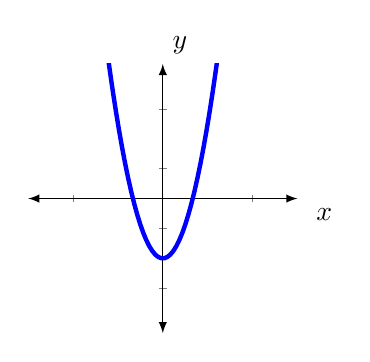
\begin{tikzpicture}[>=triangle 45,]
			\begin{axis}[
						    width = 5cm,
					               height = 5cm,
						    xmin=-4,xmax=4,
						    ymin=-4,ymax=4,
						    grid=none,
						    grid style={line width=.15pt, draw=gray!20},
						    major grid style={line width=.3pt,draw=gray!75},
						    axis lines=middle,
						    minor tick num=1,
						    enlargelimits={abs=0.5},
						    axis line style={latex-latex},
						    ticklabel style={font=\tiny,fill=white},
						    ticks=none,
						    xlabel={\,\,$x$},
						    ylabel={$y$},
						    xlabel style={below right},
						    ylabel style={above right},
						]
						\addplot+[<->, blue,samples=100, ultra thick, mark=none] {2*x^2-2};
			\end{axis}
		\end{tikzpicture}
		&
		\begin{tikzpicture}[>=triangle 45,]
			\begin{axis}[
						    width = 5cm,
					               height = 5cm,
						    xmin=-4,xmax=4,
						    ymin=-4,ymax=4,
						    grid=none,
						    grid style={line width=.15pt, draw=gray!20},
						    major grid style={line width=.3pt,draw=gray!75},
						    axis lines=middle,
						    minor tick num=1,
						    enlargelimits={abs=0.5},
						    axis line style={latex-latex},
						    ticklabel style={font=\tiny,fill=white},
						    ticks=none,
						    xlabel={\,\,$x$},
						    ylabel={$y$},
						    xlabel style={below right},
						    ylabel style={above right},
						]
						\addplot+[<->, blue,samples=100, ultra thick, mark=none] {2*x^2};
			\end{axis}
		\end{tikzpicture}
		&
		\begin{tikzpicture}[>=triangle 45,]
			\begin{axis}[
						    width = 5cm,
					               height = 5cm,
						    xmin=-4,xmax=4,
						    ymin=-4,ymax=4,
						    grid=none,
						    grid style={line width=.15pt, draw=gray!20},
						    major grid style={line width=.3pt,draw=gray!75},
						    axis lines=middle,
						    minor tick num=1,
						    enlargelimits={abs=0.5},
						    axis line style={latex-latex},
						    ticklabel style={font=\tiny,fill=white},
						    ticks=none,
						    xlabel={\,\,$x$},
						    ylabel={$y$},
						    xlabel style={below right},
						    ylabel style={above right},
						]
						\addplot+[<->, blue,samples=100, ultra thick, mark=none] {2*x^2+2};
			\end{axis}
		\end{tikzpicture}
		\\
		\hline
	\end{tabular}
\end{center}

\begin{example}
Find the type and number of solutions for each equation.
\end{example}

\begin{minipage}[t]{0.3\linewidth}
(a) $x^2-6x=-7$
\end{minipage}
\hfill
\begin{minipage}[t]{0.3\linewidth}
(b) $x^2-6x=-9$
\end{minipage}
\hfill
\begin{minipage}[t]{0.3\linewidth}
(c) $x^2-6x=-11$
\end{minipage}


\vfill
 \noindent\fbox{\large\textbf{5.6 Homework}: page 361\, 3-13 odd, 14-16 all \small }
%%%%%%%%%%%%%%%%%%%%%%%%%%%%%%%%%%%%%
%%%%%%%%%%%%%%%%%%%%%%%%%%%%%%%%%%%%%
 \newpage
%%%%%%%%%%%%%%%%%%%%%%%%%%%%%%%%%%%%%
%%%%%%%%%%%%%%%%%%%%%%%%%%%%%%%%%%%%%

\noindent \Large \textbf{TI-83/84 Quadratic Formula Program} \normalsize\\

\begin{step}
Press \tcbox[size=small, on line]{PRGM}  arrow over to \textbf{NEW} press \tcbox[size=small, on line] {ENTER}. Name the program ``QUADSOLV'' using the letters above each of the keys.
\end{step}

\vspace{-0.25cm}

\begin{step}
Once in the program press \tcbox[size=small, on line]{PRGM} and arrow over to \textbf{I/O} (input/output) and select \textbf{ClrHome}. Press \tcbox[size=small, on line]{ENTER} to start the next line. 
\end{step}

\vspace{-0.25cm}

\begin{step}
On the next line press \tcbox[size=small, on line]{PRGM} arrow over to \textbf{I/O} and select \textbf{Disp} (display) and using the \tcbox[size=small, on line]{ALPHA} key type \textbf{``}$\mathbf{AX^2+BX+C=0}$\textbf{''} in quotations. Use \tcbox[size=small, on line]{2nd} \tcbox[size=small, on line]{MATH} (TEST key) to find the equal sign ``$=$''. Press \tcbox[size=small, on line]{ENTER} to start a new line.
\end{step}

\vspace{-0.25cm}

\begin{step}
On the next line press \tcbox[size=small, on line]{PRGM} and arrow over to \textbf{I/O} and select \textbf{Prompt}. Back in the program use the  \tcbox[size=small, on line]{ALPHA} key to type \textbf{A, B, C} after the Prompt including commas. Press \tcbox[size=small, on line]{ENTER} to start the next line. 
\end{step}

\vspace{-0.25cm}

\begin{step}
On the next line type $\mathbf{B^2-4AC}$ \tcbox[size=small, on line]{STO $\mathbf{\rightarrow}$} $\mathbf{D}$.  Press \tcbox[size=small, on line]{ENTER} to start a new line.  
\end{step}

\vspace{-0.25cm}

\begin{step}
On the next line press \tcbox[size=small, on line]{MODE} and select \textbf{Float 4}. Press \tcbox[size=small, on line]{ENTER} to start a new line.
\end{step}


\begin{step}
On the next line press \tcbox[size=small, on line]{MODE} and select $\mathbf{a+bi}$. Press \tcbox[size=small, on line]{ENTER} to start a new line.
\end{step}

\vspace{-0.25cm}

\begin{step}
On the next line type $\mathbf{(-B+\sqrt{(}D))/(2A)}$  \tcbox[size=small, on line]{STO$\rightarrow$} $\mathbf{X}$.  Press \tcbox[size=small, on line]{ENTER} to start a new line.  
\end{step}

\vspace{-0.25cm}

\begin{step}
On the next line type $\mathbf{(-B-\sqrt{(}D))/(2A)}$  \tcbox[size=small, on line]{STO$\rightarrow$} $\mathbf{Y}$.  Press \tcbox[size=small, on line]{ENTER} to start a new line.  
\end{step}

\vspace{-0.25cm}

\begin{step}
On the next line press \tcbox[size=small, on line]{PRGM} arrow over to \textbf{I/O} and select \textbf{Disp}. Use the \tcbox[size=small, on line]{ALPHA} key to type \textbf{``ROOTS EQUAL:''} in quotations.
\end{step}

\vspace{-0.25cm}

\begin{step}
On the next line press \tcbox[size=small, on line]{PRGM} arrow over to \textbf{I/O} and select \textbf{Disp} and type $\mathbf{X, Y}$. 
\end{step}

\vspace{-0.25cm}

\noindent Below is the typed program as viewed from your screen.

\vspace{-0.25cm}

\begin{center}
\tcbox[size=small]{
\begin{tabular}[t]{ll}
&\texttt{PROGRAM:QUADSOLV}\\
:&\texttt{ClrHome}\\
:&$\mathtt{\texttt{Disp ``}AX^2+BX+C=0}$\texttt{''}\\
:&\texttt{Prompt A,B,C}\\
:&$\mathtt{B^2-4AC \rightarrow D}$\\
:&\texttt{Fix 4}\\
:&\texttt{a+bi}\\
:&$\mathtt{\texttt{(}-B+\sqrt{\texttt{(}}D\texttt{)}\texttt{)}/\texttt{(}2A\texttt{)} \rightarrow X}$\\
:&$\mathtt{\texttt{(}-B-\sqrt{\texttt{(}}D\texttt{)}\texttt{)}/\texttt{(}2A\texttt{)} \rightarrow Y}$\\
:&\texttt{Disp ``ROOTS EQUAL:''}\\
:&\texttt{Disp X, Y}\\
\end{tabular}
}
\end{center}

\vspace{-0.25cm}

\noindent To run the program on your calculator exit the program window by pressing  \tcbox[size=small, on line]{2nd} \tcbox[size=small, on line]{MODE} (QUIT key). You should be at the Home Screen. Press the \tcbox[size=small, on line]{PRGM} key and select \textbf{QUADSOLV} and press \tcbox[size=small, on line]{ENTER}. To test that your program runs correctly use \textbf{A=1} \textbf{B=-10} \textbf{C=29}. Your calculator should read:

\begin{center}
\tcbox[size=small]{
\begin{tabular}[t]{lr}
$\mathtt{AX^2+BX+C=0}$&\\
$\mathtt{A=?1}$&\\
$\mathtt{B=?-10}$&\\
$\mathtt{C=?29}$&\\
\texttt{ROOTS EQUAL:}&\\
&$\mathtt{5.0000+2.0000i}$\\
&$\mathtt{5.0000-2.0000i}$\\
&\texttt{Done}\\
\end{tabular}
}
\end{center}

\noindent If you get \texttt{ERR: NONREAL ANS} you may need to manually change the mode to complex numbers by pressing \tcbox[size=small, on line]{MODE} and selecting \textbf{a+bi}.

%%%%%%%%%%%%%%%%%%%%%%%%%%%%%%%%%%%%%
%%%%%%%%%%%%%%%%%%%%%%%%%%%%%%%%%%%%%
 \newpage
%%%%%%%%%%%%%%%%%%%%%%%%%%%%%%%%%%%%%
%%%%%%%%%%%%%%%%%%%%%%%%%%%%%%%%%%%%%

\noindent \Large 5.6 The Quadratic Formula (day 2) Homework \normalsize

\noindent Use your \texttt{QUADSOLV} program on your calculator to solve the problems below. 


\noindent Find the zeros of each function by using the Quadratic Formula.

\begin{enumerate}

\begin{minipage}[t]{0.45\linewidth}
\item  $f(x)=3x^2-10x+3$\\
\end{minipage}
\hfill
\begin{minipage}[t]{0.45\linewidth}
\item  $g(x)=x^2+6x$\\
\end{minipage}

\vspace{1cm}
%%

\begin{minipage}[t]{0.45\linewidth}
\item  $h(x)=x(x-3)-4$\\
\end{minipage}
\hfill
\begin{minipage}[t]{0.45\linewidth}
\item  $g(x)=-x^2-2x+9$\\
\end{minipage}

\vspace{1cm}
%%

\begin{minipage}[t]{0.45\linewidth}
\item  $p(x)=2x^2-7x-8$\\
\end{minipage}
\hfill
\begin{minipage}[t]{0.45\linewidth}
\item  $f(x)=7x^2-3$\\
\end{minipage}

\vspace{1cm}
%%

\begin{minipage}[t]{0.45\linewidth}
\item  $r(x)=x^2+x+1$\\
\end{minipage}
\hfill
\begin{minipage}[t]{0.45\linewidth}
\item  $h(x)=-x^2-x-1$\\
\end{minipage}

\vspace{1cm}
%%

\begin{minipage}[t]{0.45\linewidth}
\item  $f(x)=2x^2+8$\\
\end{minipage}
\hfill
\begin{minipage}[t]{0.45\linewidth}
\item  $f(x)=2x^2+7x-13$\\
\end{minipage}

\vspace{0.5cm}
%%

\end{enumerate}

\noindent Find the type and number of solutions for each equation.

\begin{enumerate}
\setcounter{enumi}{10}

\begin{minipage}[t]{0.45\linewidth}
\item  $2x^2+5=2x$
\end{minipage}
\hfill
\begin{minipage}[t]{0.45\linewidth}
\item  $2x^2-3x=8$
\end{minipage}

\vspace{1cm}
%%

\begin{minipage}[t]{0.45\linewidth}
\item $2x^2-16x=-32$
\end{minipage}
\hfill
\begin{minipage}[t]{0.45\linewidth}
\item $4x^2-28x=-49$
\end{minipage}

\vspace{1cm}
%%

\end{enumerate}

\noindent Solve each equation by any method.

\begin{enumerate}
\setcounter{enumi}{14}

\begin{minipage}[t]{0.45\linewidth}
\item  $x^2=7$
\end{minipage}
\hfill
\begin{minipage}[t]{0.45\linewidth}
\item  $x^2-4x-21=0$
\end{minipage}

\vspace{1cm}
%%

\begin{minipage}[t]{0.45\linewidth}
\item $6x^2=150$
\end{minipage}
\hfill
\begin{minipage}[t]{0.45\linewidth}
\item $4x^2-4x-1=0$
\end{minipage}

\vspace{1cm}
%%

\end{enumerate}


\hrule

\vfill
\small
\color{red}
\begin{flushright}
\rotatebox{180}{ 16. $x=-3, 7$\, 17. $x=\pm 5$\, 18. 1.2071, -0.2071 \, }\\
\rotatebox{180}{ 11. Two non-real\, 12. Two non-real\, 13. One real\, 14. One real\, 15. $x=\pm i\sqrt{7}=\pm 2.6458i$\,  }\\
\rotatebox{180}{ 6. $x=\pm 0.6547, $\, 7. $x=-0.5\pm 0.8660i$\, 8. $x=-0.5\pm 0.8660i$\,  9. $x=\pm 2i$\, 10. $x=1.3423, -4.8423$\, }\\
\rotatebox{180}{Solutions: 1. $x= 3, 0.3333$\, 2. $x=0, -6$\, 3. $x=4, -1$\, 4. $x=-4.1623, 2.1623 $\, 5. $x=4.4075, -0.9075$\,  }
\end{flushright}
\color{black}
\normalsize

%%%%%%%%%%%%%%%%%%%%%%%%%%%%%%%%%%%%%
%%%%%%%%%%%%%%%%%%%%%%%%%%%%%%%%%%%%%
 \newpage
%%%%%%%%%%%%%%%%%%%%%%%%%%%%%%%%%%%%%
%%%%%%%%%%%%%%%%%%%%%%%%%%%%%%%%%%%%%

%%%%%%%%%%%%%%%%%%%%%%%%%%%%%%%
%%%%%%%%%%%%%%%%%%%%%%%%%%%%%%%
%%%%%%   Section 5.7   %%%%%%%%
%%%%%%%%%%%%%%%%%%%%%%%%%%%%%%%
%%%%%%%%%%%%%%%%%%%%%%%%%%%%%%%
 \section{  Solving Quadratic Inequalities }
 \setcounter{example}{0}
 \setcounter{definition}{0}
 \hfill \underline{Objective}: Solve quadratic inequalities by using tables and graphs. \\
 %%%%%%%%%%%%%%%%%%%%%%%%%%%%%%%%
 %%%%%%%%%%%%%%%%%%%%%%%%%%%%%%%%
 \begin{definition}
 A \textbf{quadratic inequality in two variables} can be written in one of the following forms, where $a$, $b$, and $c$ are real numbers and $a\neq 0$. Its solution set is a set of ordered pairs $(x,y)$ so that:
 \end{definition}
 \vspace{-1cm}
 
\hfill
\begin{minipage}[t]{0.3\linewidth}
 \[y<ax^2+bx+c\]
 \[y\leq ax^2+bx+c\]
\end{minipage}
\begin{minipage}[t]{0.3\linewidth}
 \[y> ax^2+bx+c\]
 \[y\geq ax^2+bx+c\]
\end{minipage}\hfill
\hfill
 
 \vspace{-0.5cm}
 
 \begin{center}
	 \begin{tabular}[t]{|l|l|}
	 	\hline
	 	 \multicolumn{2}{|c|}{}\\
		 \multicolumn{2}{|c|}{\textbf{Graphing Quadratic Inequalities}}\\
		 \hline
		 &\multirow{3}{*}{
		 	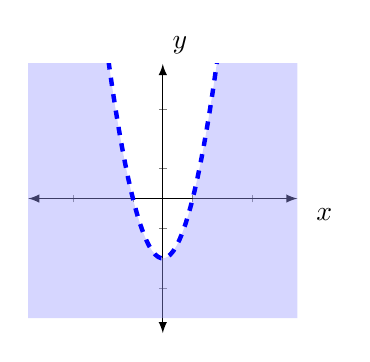
\begin{tikzpicture}[>=triangle 45,]
				\begin{axis}[
							    width = 5cm,
						               height = 5cm,
							    xmin=-4,xmax=4,
							    ymin=-4,ymax=4,
							    grid=none,
							    grid style={line width=.15pt, draw=gray!20},
							    major grid style={line width=.3pt,draw=gray!75},
							    axis lines=middle,
							    minor tick num=1,
							    enlargelimits={abs=0.5},
							    axis line style={latex-latex},
							    ticklabel style={font=\tiny,fill=white},
							    ticks=none,
							    xlabel={\,\,$x$},
							    ylabel={$y$},
							    xlabel style={below right},
							    ylabel style={above right},
							]
							\addplot+[<->,dashed,  blue,samples=100, ultra thick, mark=none, name path=A] {2*x^2-2};
							\addplot+[-, blue, ultra thin, name path = B, mark=none, opacity =0] { -4};
							\addplot+[blue!40, opacity =0.4] fill between [of= A and B];
				\end{axis}
			\end{tikzpicture}}\\
		 \textbf{To graph a quadratic inequality}&\\
		\cline{1-1}
		&\\
		 1. Graph the parabola that defines the boundary.&\\
		 \cline{1-1}
		 &\\
		 2. Use a solid parabola for $y\leq$ and $y\geq$ and a dashed  &\\
		 parabola for $y<$ and $y>$.&\\
		 \cline{1-1}
		 &\\
		 3. Shade above the parabola for $y>$ or $\geq$ and below the&\\
		 parabola for $y\leq$ or $<$.&\\
		 \hline
	 \end{tabular}
 \end{center}
 
 \begin{example}
 Graph each of the following quadratic inequalities.
 \end{example}

\vspace{-0.5cm}


\begin{minipage}[t]{0.45\linewidth}
(a) $y\leq -2x^2-4x+6$\\
	 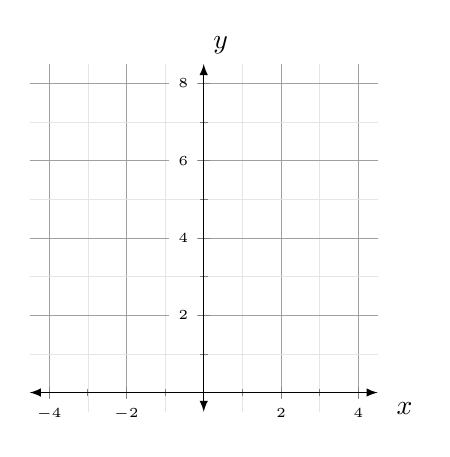
\begin{tikzpicture}[>=latex]
			\begin{axis}[
					    width =6cm,
				               height=6cm,
					    xmin=-4,xmax=4,
					    ymin=0,ymax=8,
					    grid=both,
					    grid style={line width=.15pt, draw=gray!20},
					    major grid style={line width=.3pt,draw=gray!75},
					    axis lines=middle,
					    minor tick num=1,
					    enlargelimits={abs=0.5},
					    axis line style={latex-latex},
					    ticklabel style={font=\tiny,fill=white},
					    xlabel={\,\,$x$},
					    ylabel={$y$},
					    xlabel style={below right},
					    ylabel style={above right},
					]
			\end{axis}
			%\draw[color=blue,thick] plot (\x,\x*\x);
	\end{tikzpicture}
\end{minipage}
\hfill
\begin{minipage}[t]{0.45\linewidth}
(b) $y\geq x^2-2x+1$ \\
	 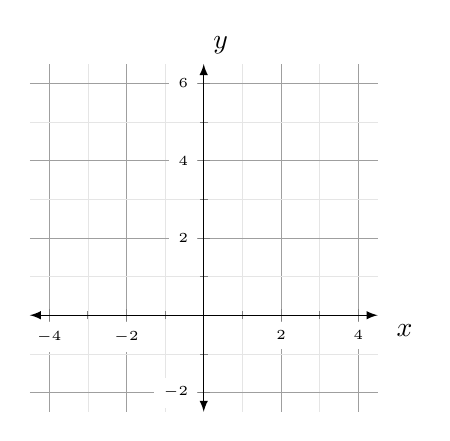
\begin{tikzpicture}[>=latex]
			\begin{axis}[
					    width =6cm,
				               height=6cm,
					    xmin=-4,xmax=4,
					    ymin=-2,ymax=6,
					    grid=both,
					    grid style={line width=.15pt, draw=gray!20},
					    major grid style={line width=.3pt,draw=gray!75},
					    axis lines=middle,
					    minor tick num=1,
					    enlargelimits={abs=0.5},
					    axis line style={latex-latex},
					    ticklabel style={font=\tiny,fill=white},
					    xlabel={\,\,$x$},
					    ylabel={$y$},
					    xlabel style={below right},
					    ylabel style={above right},
					]
			\end{axis}
			%\draw[color=blue,thick] plot (\x,\x*\x);
	\end{tikzpicture}
\end{minipage}

\begin{minipage}[t]{0.3\linewidth}
(c) $y<x^2-6x+8$ \\
	 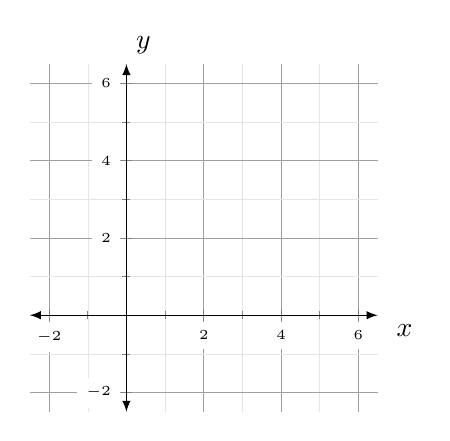
\begin{tikzpicture}[>=latex]
			\begin{axis}[
					    width =6cm,
				               height=6cm,
					    xmin=-2,xmax=6,
					    ymin=-2,ymax=6,
					    grid=both,
					    grid style={line width=.15pt, draw=gray!20},
					    major grid style={line width=.3pt,draw=gray!75},
					    axis lines=middle,
					    minor tick num=1,
					    enlargelimits={abs=0.5},
					    axis line style={latex-latex},
					    ticklabel style={font=\tiny,fill=white},
					    xlabel={\,\,$x$},
					    ylabel={$y$},
					    xlabel style={below right},
					    ylabel style={above right},
					]
			\end{axis}
			%\draw[color=blue,thick] plot (\x,\x*\x);
	\end{tikzpicture}
\end{minipage}
\hfill
\begin{minipage}[t]{0.45\linewidth}
(d) $y>-x^2-2x+3$ \\
	 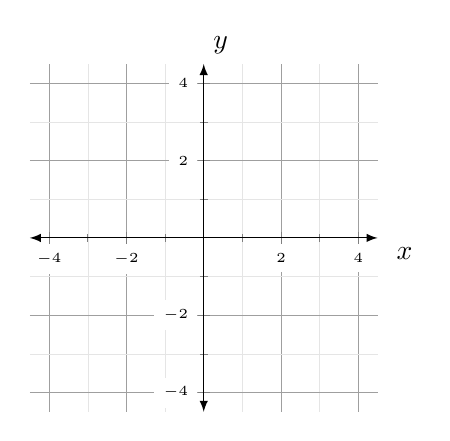
\begin{tikzpicture}[>=latex]
			\begin{axis}[
					    width =6cm,
				               height=6cm,
					    xmin=-4,xmax=4,
					    ymin=-4,ymax=4,
					    grid=both,
					    grid style={line width=.15pt, draw=gray!20},
					    major grid style={line width=.3pt,draw=gray!75},
					    axis lines=middle,
					    minor tick num=1,
					    enlargelimits={abs=0.5},
					    axis line style={latex-latex},
					    ticklabel style={font=\tiny,fill=white},
					    xlabel={\,\,$x$},
					    ylabel={$y$},
					    xlabel style={below right},
					    ylabel style={above right},
					]
			\end{axis}
			%\draw[color=blue,thick] plot (\x,\x*\x);
	\end{tikzpicture}
\end{minipage}

%%%%%%%%%%%%%%%%%%%%%%%%%%%%%%%%%%%%%
%%%%%%%%%%%%%%%%%%%%%%%%%%%%%%%%%%%%%
 \newpage
%%%%%%%%%%%%%%%%%%%%%%%%%%%%%%%%%%%%%
%%%%%%%%%%%%%%%%%%%%%%%%%%%%%%%%%%%%%

\begin{example}
Solve the inequalities using algebra.
\end{example}

\begin{minipage}[t]{0.45\linewidth}
(a) $x^2-4x+1>6$\\


\vspace{4cm}
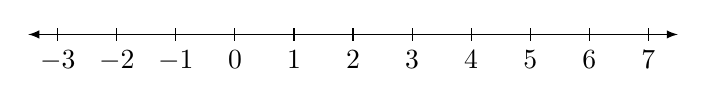
\begin{tikzpicture}[scale=0.75]
        \draw[latex-latex] (-3.5,0) -- (7.5,0) ; %edit here for the axis
        \foreach \x in  {-3,-2,-1,0,1,2,3,4,5,6,7} % edit here for the vertical lines
        \draw[shift={(\x,0)},color=black] (0pt,3pt) -- (0pt,-3pt);
        \foreach \x in {-3,-2,-1,0,1,2,3,4,5,6,7} % edit here for the numbers
        \draw[shift={(\x,0)},color=black] (0pt,0pt) -- (0pt,-3pt) node[below] {$\x$};
\end{tikzpicture}
\vspace{1cm}

(c) $x^2-6x+8\leq 3$ \\

\vspace{4cm}
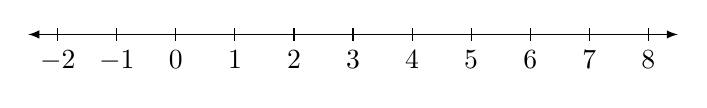
\begin{tikzpicture}[scale=0.75]
        \draw[latex-latex] (-2.5,0) -- (8.5,0) ; %edit here for the axis
        \foreach \x in  {-2,-1,0,1,2,3,4,5,6,7,8} % edit here for the vertical lines
        \draw[shift={(\x,0)},color=black] (0pt,3pt) -- (0pt,-3pt);
        \foreach \x in {-2,-1,0,1,2,3,4,5,6,7,8} % edit here for the numbers
        \draw[shift={(\x,0)},color=black] (0pt,0pt) -- (0pt,-3pt) node[below] {$\x$};
\end{tikzpicture}
\vspace{1cm}

\end{minipage}
\hfill
\begin{minipage}[t]{0.45\linewidth}
(b) $x^2-x+5<7$ \\

\vspace{4cm}
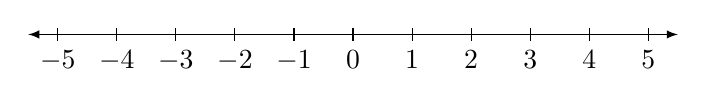
\begin{tikzpicture}[scale=0.75]
        \draw[latex-latex] (-5.5,0) -- (5.5,0) ; %edit here for the axis
        \foreach \x in  {-5,-4,-3,-2,-1,0,1,2,3,4,5} % edit here for the vertical lines
        \draw[shift={(\x,0)},color=black] (0pt,3pt) -- (0pt,-3pt);
        \foreach \x in {-5,-4,-3,-2,-1,0,1,2,3,4,5} % edit here for the numbers
        \draw[shift={(\x,0)},color=black] (0pt,0pt) -- (0pt,-3pt) node[below] {$\x$};
\end{tikzpicture}
\vspace{1cm}

(d) $-2x^2+3x+7<2$ \\

\vspace{4cm}
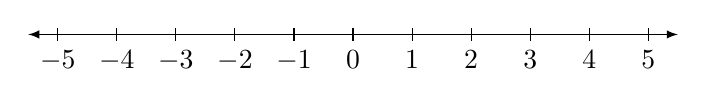
\begin{tikzpicture}[scale=0.75]
        \draw[latex-latex] (-5.5,0) -- (5.5,0) ; %edit here for the axis
        \foreach \x in  {-5,-4,-3,-2,-1,0,1,2,3,4,5} % edit here for the vertical lines
        \draw[shift={(\x,0)},color=black] (0pt,3pt) -- (0pt,-3pt);
        \foreach \x in {-5,-4,-3,-2,-1,0,1,2,3,4,5} % edit here for the numbers
        \draw[shift={(\x,0)},color=black] (0pt,0pt) -- (0pt,-3pt) node[below] {$\x$};
\end{tikzpicture}
\vspace{1cm}
\end{minipage}

\begin{youtry}
Solve the inequalities using algebra.
\end{youtry}

\begin{minipage}[t]{0.45\linewidth}
(a) $x^2-6x+10\geq 2$\\

\vspace{4cm}
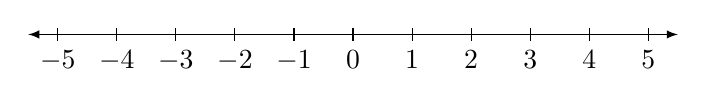
\begin{tikzpicture}[scale=0.75]
        \draw[latex-latex] (-5.5,0) -- (5.5,0) ; %edit here for the axis
        \foreach \x in  {-5,-4,-3,-2,-1,0,1,2,3,4,5} % edit here for the vertical lines
        \draw[shift={(\x,0)},color=black] (0pt,3pt) -- (0pt,-3pt);
        \foreach \x in {-5,-4,-3,-2,-1,0,1,2,3,4,5} % edit here for the numbers
        \draw[shift={(\x,0)},color=black] (0pt,0pt) -- (0pt,-3pt) node[below] {$\x$};
\end{tikzpicture}
\vspace{1cm}
\end{minipage}
\hfill
\begin{minipage}[t]{0.45\linewidth}
(b) $x^2-1<3$ \\

\vspace{4cm}
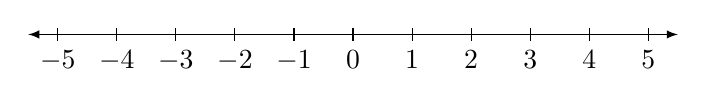
\begin{tikzpicture}[scale=0.75]
        \draw[latex-latex] (-5.5,0) -- (5.5,0) ; %edit here for the axis
        \foreach \x in  {-5,-4,-3,-2,-1,0,1,2,3,4,5} % edit here for the vertical lines
        \draw[shift={(\x,0)},color=black] (0pt,3pt) -- (0pt,-3pt);
        \foreach \x in {-5,-4,-3,-2,-1,0,1,2,3,4,5} % edit here for the numbers
        \draw[shift={(\x,0)},color=black] (0pt,0pt) -- (0pt,-3pt) node[below] {$\x$};
\end{tikzpicture}
\vspace{1cm}

\end{minipage}




\vfill
 \noindent\fbox{\large\textbf{5.7 Homework}: page 370 \, 2-4, 8-10, 13-21 odds \small }
%%%%%%%%%%%%%%%%%%%%%%%%%%%%%%%%%%%%%
%%%%%%%%%%%%%%%%%%%%%%%%%%%%%%%%%%%%%
 \newpage
%%%%%%%%%%%%%%%%%%%%%%%%%%%%%%%%%%%%%
%%%%%%%%%%%%%%%%%%%%%%%%%%%%%%%%%%%%%


 \noindent\Large {\textbf{ 5.7 Solving Quadratic Inequalities Homework (day 2)} }
 \setcounter{example}{0}
 \setcounter{definition}{0}
\\
\small\indent\,\hfill\underline{Objective}: Solve quadratic inequalities by using tables and graphs.\normalsize \\
 %%%%%%%%%%%%%%%%%%%%%%%%%%%%%%%%
 %%%%%%%%%%%%%%%%%%%%%%%%%%%%%%%%


\vspace{-1.35cm}


 \noindent Graph each of the following quadratic inequalities.
\begin{enumerate}


\begin{minipage}[t]{0.45\linewidth}
\item $y\geq2x^2$\\
	 \begin{tikzpicture}[>=latex]
			\begin{axis}[
					    width =6cm,
				               height=6cm,
					    xmin=-4,xmax=4,
					    ymin=-2,ymax=6,
					    grid=both,
					    grid style={line width=.15pt, draw=gray!20},
					    major grid style={line width=.3pt,draw=gray!75},
					    axis lines=middle,
					    minor tick num=1,
					    enlargelimits={abs=0.5},
					    axis line style={latex-latex},
					    ticklabel style={font=\tiny,fill=white},
					    xlabel={\,\,$x$},
					    ylabel={$y$},
					    xlabel style={below right},
					    ylabel style={above right},
					]
			\end{axis}
			%\draw[color=blue,thick] plot (\x,\x*\x);
	\end{tikzpicture}
\end{minipage}
\hfill
\begin{minipage}[t]{0.45\linewidth}
\item $y > 3x^2$ \\
	 \begin{tikzpicture}[>=latex]
			\begin{axis}[
					    width =6cm,
				               height=6cm,
					    xmin=-4,xmax=4,
					    ymin=-2,ymax=6,
					    grid=both,
					    grid style={line width=.15pt, draw=gray!20},
					    major grid style={line width=.3pt,draw=gray!75},
					    axis lines=middle,
					    minor tick num=1,
					    enlargelimits={abs=0.5},
					    axis line style={latex-latex},
					    ticklabel style={font=\tiny,fill=white},
					    xlabel={\,\,$x$},
					    ylabel={$y$},
					    xlabel style={below right},
					    ylabel style={above right},
					]
			\end{axis}
			%\draw[color=blue,thick] plot (\x,\x*\x);
	\end{tikzpicture}
\end{minipage}

\begin{minipage}[t]{0.3\linewidth}
\item $y\leq -x^2$ \\
	 \begin{tikzpicture}[>=latex]
			\begin{axis}[
					    width =6cm,
				               height=6cm,
					    xmin=-4,xmax=4,
					    ymin=-6,ymax=2,
					    grid=both,
					    grid style={line width=.15pt, draw=gray!20},
					    major grid style={line width=.3pt,draw=gray!75},
					    axis lines=middle,
					    minor tick num=1,
					    enlargelimits={abs=0.5},
					    axis line style={latex-latex},
					    ticklabel style={font=\tiny,fill=white},
					    xlabel={\,\,$x$},
					    ylabel={$y$},
					    xlabel style={below right},
					    ylabel style={above right},
					]
			\end{axis}
			%\draw[color=blue,thick] plot (\x,\x*\x);
	\end{tikzpicture}
\end{minipage}
\hfill
\begin{minipage}[t]{0.45\linewidth}
\item $y < -2x^2-8x-12$ \\
	 \begin{tikzpicture}[>=latex]
			\begin{axis}[
					    width =6cm,
				               height=6cm,
					    xmin=-4,xmax=4,
					    ymin=-8,ymax=0,
					    grid=both,
					    grid style={line width=.15pt, draw=gray!20},
					    major grid style={line width=.3pt,draw=gray!75},
					    axis lines=middle,
					    minor tick num=1,
					    enlargelimits={abs=0.5},
					    axis line style={latex-latex},
					    ticklabel style={font=\tiny,fill=white},
					    xlabel={\,\,$x$},
					    ylabel={$y$},
					    xlabel style={below right},
					    ylabel style={above right},
					]
			\end{axis}
			%\draw[color=blue,thick] plot (\x,\x*\x);
	\end{tikzpicture}
\end{minipage}


\begin{minipage}[t]{0.45\linewidth}
\item $y\leq x^2-6x+11$\\
	 \begin{tikzpicture}[>=latex]
			\begin{axis}[
					    width =6cm,
				               height=6cm,
					    xmin=-2,xmax=6,
					    ymin=0,ymax=8,
					    grid=both,
					    grid style={line width=.15pt, draw=gray!20},
					    major grid style={line width=.3pt,draw=gray!75},
					    axis lines=middle,
					    minor tick num=1,
					    enlargelimits={abs=0.5},
					    axis line style={latex-latex},
					    ticklabel style={font=\tiny,fill=white},
					    xlabel={\,\,$x$},
					    ylabel={$y$},
					    xlabel style={below right},
					    ylabel style={above right},
					]
			\end{axis}
			%\draw[color=blue,thick] plot (\x,\x*\x);
	\end{tikzpicture}
\end{minipage}
\hfill
\begin{minipage}[t]{0.45\linewidth}
\item $y \geq -2x^2+16x-29  $ \\
	 \begin{tikzpicture}[>=latex]
			\begin{axis}[
					    width =6cm,
				               height=6cm,
					    xmin=0,xmax=6,
					    ymin=-2,ymax=4,
					    grid=both,
					    grid style={line width=.15pt, draw=gray!20},
					    major grid style={line width=.3pt,draw=gray!75},
					    axis lines=middle,
					    minor tick num=1,
					    enlargelimits={abs=0.5},
					    axis line style={latex-latex},
					    ticklabel style={font=\tiny,fill=white},
					    xlabel={\,\,$x$},
					    ylabel={$y$},
					    xlabel style={below right},
					    ylabel style={above right},
					]
			\end{axis}
			%\draw[color=blue,thick] plot (\x,\x*\x);
	\end{tikzpicture}
\end{minipage}

\begin{minipage}[t]{0.3\linewidth}
\item $y>-x^2+4x+11$ \\
	 \begin{tikzpicture}[>=latex]
			\begin{axis}[
					    width =6cm,
				               height=6cm,
					    xmin=-2,xmax=6,
					    ymin=-8,ymax=0,
					    grid=both,
					    grid style={line width=.15pt, draw=gray!20},
					    major grid style={line width=.3pt,draw=gray!75},
					    axis lines=middle,
					    minor tick num=1,
					    enlargelimits={abs=0.5},
					    axis line style={latex-latex},
					    ticklabel style={font=\tiny,fill=white},
					    xlabel={\,\,$x$},
					    ylabel={$y$},
					    xlabel style={below right},
					    ylabel style={above right},
					]
			\end{axis}
			%\draw[color=blue,thick] plot (\x,\x*\x);
	\end{tikzpicture}
\end{minipage}
\hfill
\begin{minipage}[t]{0.45\linewidth}
\item $y>-2x^2+16x-34$ \\
	 \begin{tikzpicture}[>=latex]
			\begin{axis}[
					    width =6cm,
				               height=6cm,
					    xmin=0,xmax=8,
					    ymin=-9,ymax=0,
					    grid=both,
					    grid style={line width=.15pt, draw=gray!20},
					    major grid style={line width=.3pt,draw=gray!75},
					    axis lines=middle,
					    minor tick num=1,
					    enlargelimits={abs=0.5},
					    axis line style={latex-latex},
					    ticklabel style={font=\tiny,fill=white},
					    xlabel={\,\,$x$},
					    ylabel={$y$},
					    xlabel style={below right},
					    ylabel style={above right},
					]
			\end{axis}
			%\draw[color=blue,thick] plot (\x,\x*\x);
	\end{tikzpicture}
\end{minipage}

\end{enumerate}

%%%%%%%%%%%%%%%%%%%%%%%%%%%%%%%%%%%%%
%%%%%%%%%%%%%%%%%%%%%%%%%%%%%%%%%%%%%
 \newpage
%%%%%%%%%%%%%%%%%%%%%%%%%%%%%%%%%%%%%
%%%%%%%%%%%%%%%%%%%%%%%%%%%%%%%%%%%%%


\noindent Solve the inequalities using using any method.\\ 
\noindent Write your answer on the \textbf{number line} and in \textbf{interval notation}.\\

\begin{enumerate}
\setcounter{enumi}{8}


\begin{minipage}[t]{0.45\linewidth}

\vspace{0.5cm}

\item $x^2-3x-10<0$\\


\vspace{4cm}
\begin{tikzpicture}[scale=0.7]
        \draw[latex-latex] (-4.5,0) -- (6.5,0) ; %edit here for the axis
        \foreach \x in  { -4,-3,-2,-1,0,1,2,3,4,5,6} % edit here for the vertical lines
        \draw[shift={(\x,0)},color=black] (0pt,3pt) -- (0pt,-3pt);
        \foreach \x in {-4,-3,-2,-1,0,1,2,3,4,5,6} % edit here for the numbers
        \draw[shift={(\x,0)},color=black] (0pt,0pt) -- (0pt,-3pt) node[below] {$\x$};
\end{tikzpicture}
\vspace{1cm}

\setcounter{enumi}{10}
\item $-x^2+x+6>0$ \\

\vspace{4cm}
\begin{tikzpicture}[scale=0.7]
        \draw[latex-latex] (-4.5,0) -- (4.5,0) ; %edit here for the axis
        \foreach \x in  { -4,-3,-2,-1,0,1,2,3,4} % edit here for the vertical lines
        \draw[shift={(\x,0)},color=black] (0pt,3pt) -- (0pt,-3pt);
        \foreach \x in {-4,-3,-2,-1,0,1,2,3,4} % edit here for the numbers
        \draw[shift={(\x,0)},color=black] (0pt,0pt) -- (0pt,-3pt) node[below] {$\x$};
\end{tikzpicture}
\vspace{1cm}

\end{minipage}
\hfill
\begin{minipage}[t]{0.45\linewidth}

\vspace{0.5cm}

\setcounter{enumi}{9}
\item $x^2-3x-4<0$ \\

\vspace{4cm}
\begin{tikzpicture}[scale=0.7]
        \draw[latex-latex] (-3.5,0) -- (5.5,0) ; %edit here for the axis
        \foreach \x in  {-3,-2,-1,0,1,2,3,4,5} % edit here for the vertical lines
        \draw[shift={(\x,0)},color=black] (0pt,3pt) -- (0pt,-3pt);
        \foreach \x in {-3,-2,-1,0,1,2,3,4,5} % edit here for the numbers
        \draw[shift={(\x,0)},color=black] (0pt,0pt) -- (0pt,-3pt) node[below] {$\x$};
\end{tikzpicture}
\vspace{1.5cm}

\setcounter{enumi}{11}
\item $x^2+3x\geq 10$ \\

\vspace{4cm}
\begin{tikzpicture}[scale=0.7]
        \draw[latex-latex] (-6.5,0) -- (4.5,0) ; %edit here for the axis
        \foreach \x in  {-6, -5, -4,-3,-2,-1,0,1,2,3,4} % edit here for the vertical lines
        \draw[shift={(\x,0)},color=black] (0pt,3pt) -- (0pt,-3pt);
        \foreach \x in {-6,-5,-4,-3,-2,-1,0,1,2,3,4} % edit here for the numbers
        \draw[shift={(\x,0)},color=black] (0pt,0pt) -- (0pt,-3pt) node[below] {$\x$};
\end{tikzpicture}
\vspace{1cm}
\end{minipage}



\begin{minipage}[t]{0.45\linewidth}
\item $x^2-12\leq -x$\\

\vspace{4cm}
\begin{tikzpicture}[scale=0.7]
        \draw[latex-latex] (-5.5,0) -- (5.5,0) ; %edit here for the axis
        \foreach \x in  { -5, -4,-3,-2,-1,0,1,2,3,4,5} % edit here for the vertical lines
        \draw[shift={(\x,0)},color=black] (0pt,3pt) -- (0pt,-3pt);
        \foreach \x in {-5,-4,-3,-2,-1,0,1,2,3,4,5} % edit here for the numbers
        \draw[shift={(\x,0)},color=black] (0pt,0pt) -- (0pt,-3pt) node[below] {$\x$};
\end{tikzpicture}
\vspace{1.5cm}
\end{minipage}
\hfill
\begin{minipage}[t]{0.45\linewidth}
\item $x^2+x-2>0$ \\

\vspace{4cm}
\begin{tikzpicture}[scale=0.7]
        \draw[latex-latex] (-3.5,0) -- (3.5,0) ; %edit here for the axis
        \foreach \x in  {-3,-2,-1,0,1,2,3} % edit here for the vertical lines
        \draw[shift={(\x,0)},color=black] (0pt,3pt) -- (0pt,-3pt);
        \foreach \x in {-3,-2,-1,0,1,2,3} % edit here for the numbers
        \draw[shift={(\x,0)},color=black] (0pt,0pt) -- (0pt,-3pt) node[below] {$\x$};
\end{tikzpicture}
\vspace{1cm}

\end{minipage}

\end{enumerate}


%%%%%%%%%%%%%%%%%%%%%%%%%%%%%%%%%%%%%%%
%%%%%%%%  ADD SOLUTIONS HERE (ODDS ON PAGE 371) %%%%%%%%%%
%%%%%%%%%%%%%%%%%%%%%%%%%%%%%%%%%%%%%%%






%%%%%%%%%%%%%%%%%%%%%%%%%%%%%%%%%%%%%
%%%%%%%%%%%%%%%%%%%%%%%%%%%%%%%%%%%%%
 \newpage
%%%%%%%%%%%%%%%%%%%%%%%%%%%%%%%%%%%%%
%%%%%%%%%%%%%%%%%%%%%%%%%%%%%%%%%%%%%


%%%%%%%%%%%%%%%%%%%%%%%%%%%%%%%
%%%%%%%%%%%%%%%%%%%%%%%%%%%%%%%
%%%%%%   Section 5.8   %%%%%%%%
%%%%%%%%%%%%%%%%%%%%%%%%%%%%%%%
%%%%%%%%%%%%%%%%%%%%%%%%%%%%%%%
 \section{ Curve Fitting with Quadratic  }
 \setcounter{example}{0}
 \setcounter{definition}{0}
 \vspace{-0.5cm}
 
 \hfill \underline{Objective}: Use quadratic functions to model data.\\
 %%%%%%%%%%%%%%%%%%%%%%%%%%%%%%%%
 %%%%%%%%%%%%%%%%%%%%%%%%%%%%%%%%
 
 \vspace{-1cm}
 
\begin{center}
	\begin{tabular}[t]{|c|c|c|c|c|c|c|c|}
		\hline
		&&&&&&&\\
		$x$&-3&-2&-1&0&1&2&3\\
		\hline
		&&&&&&&\\
		$f(x)=x^2$&9&4&1&0&1&4&9\\
		\hline
		\multicolumn{8}{c}{}\\
		\multicolumn{1}{c}{\color{blue} 1st differences} & \multicolumn{7}{c}{\color{blue} -5\,\,\quad-3\,\,\quad-1\,\,\quad1\,\,\quad3\,\,\quad5}\\
		\multicolumn{1}{c}{\color{red} 2nd differences} & \multicolumn{7}{c}{\color{red} 2 \,\,\quad 2\,\,\,\quad 2\,\,\,\quad 2\,\,\quad 2}\\
		\multicolumn{8}{c}{}\\
		\multicolumn{1}{c}{}&\multicolumn{7}{c}{\color{red} Constant 2nd Differences}\\
	\end{tabular}
\end{center}


 \begin{example}
 Determined whether each data set could represent a quadratic function. Explain.
 \end{example}

\begin{minipage}[t]{0.45\linewidth}
(a)\\

\vspace{-1.75cm}

\begin{center} 
\begin{tabular}[t]{|c|c|c|c|c|c|c|}
\hline
$x$&0&2&4&6&8\\
\hline
$y$&12&10&9&9&10\\
\hline
\end{tabular}
\end{center}
\end{minipage}
\hfill
\begin{minipage}[t]{0.45\linewidth}
(b)\\

\vspace{-1.75cm}

\begin{center}
\begin{tabular}[t]{|c|c|c|c|c|c|c|}
\hline
$x$&-2&-1&0&1&2\\
\hline
$y$&1&2&4&8&16\\
\hline
\end{tabular}
\end{center}
\end{minipage}


\vspace{2.5cm}


 \begin{youtry}
 Determined whether each data set could represent a quadratic function. Explain.
 \end{youtry}

\begin{minipage}[t]{0.45\linewidth}
(a) \\

\vspace{-1.75cm}

\begin{center}
	\begin{tabular}[t]{|c|c|c|c|c|c|c|}
	\hline
	$x$&3&4&5&6&7\\
	\hline
	$y$&11&21&35&53&75\\
	\hline
	\end{tabular}
\end{center}
\end{minipage}
\hfill
\begin{minipage}[t]{0.45\linewidth}
(b)\\

\vspace{-1.75cm}

\begin{center}
\begin{tabular}[t]{|c|c|c|c|c|c|c|}
\hline
$x$&10&9&8&7&6\\
\hline
$y$&6&8&10&12&14\\
\hline
\end{tabular}
\end{center}
\end{minipage}

\vspace{2.5cm}


\begin{definition}
A \textbf{quadratic model} is a quadratic function that represents a real data set. Models are useful for making estimates.You can apply statistical methods to make a quadratic model for a given data set using \textbf{quadratic regression}.\\
\end{definition}

\large\noindent\textbf{Quadratic Regression on TI-Calculator}\normalsize\\

\vspace{-0.5cm}
\noindent \underline{Step 1}: Enter data into your TI-83/84 graphing calculator by selecting \tcbox[size=small, on line]{STAT} and select \texttt{1:Edit$\ldots$}. Enter the  all the $x$-coordinates in the list \texttt{L1} and all the corresponding $y$-coordinates in the \texttt{L2}.

\vspace{-0.35cm}
\noindent \underline{Step 2}: Select \tcbox[size=small, on line]{STAT} arrow over to \texttt{CALC} and arrow down to \texttt{5:QuadReg}. Next press \tcbox[size=small, on line]{2nd} \tcbox[size=small, on line]{STAT} (\texttt{LIST} button) and select \texttt{L1} press \tcbox[size=small, on line]{,} and again press \tcbox[size=small, on line]{2nd} \tcbox[size=small, on line]{STAT} (\texttt{LIST}) select \texttt{L2} and finally press \tcbox[size=small, on line]{ENTER}. Write down the the quadratic using coefficents $a$, $b$, and $c$.

\vspace{-0.35cm}
\noindent \underline{Step 3}: Press \tcbox[size=small, on line]{2nd} \tcbox[size=small, on line]{$y=$} (\texttt{STAT PLOT} button). Select \texttt{1:Plot1$\ldots$Off}. Arrow over \texttt{On} and select it. Arrow down to \texttt{YList:} and press \tcbox[size=small, on line]{2nd} \tcbox[size=small, on line]{STAT} (\texttt{LIST}) and select \texttt{L2}. On TI-83 you want to use \tcbox[size=small, on line]{2nd} \tcbox[size=small, on line]{1} to get \texttt{L1} and \tcbox[size=small, on line]{2nd} \tcbox[size=small, on line]{2} to get \texttt{L2}.

\vspace{-0.35cm}
\noindent \underline{Step 4}: Press \tcbox[size=small, on line]{$y=$} and type the quadratic equation found in Step 2 using the coefficents. Next press \tcbox[size=small, on line]{GRAPH}.

%%%%%%%%%%%%%%%%%%%%%%%%%%%%%%%%%%%%%
%%%%%%%%%%%%%%%%%%%%%%%%%%%%%%%%%%%%%
 \newpage
%%%%%%%%%%%%%%%%%%%%%%%%%%%%%%%%%%%%%
%%%%%%%%%%%%%%%%%%%%%%%%%%%%%%%%%%%%%




\begin{example}
Write a quadratic function that fits each set of points.
\end{example}

\begin{minipage}[t]{0.45\linewidth}
(a)  $(0,5)$, $(2,1)$, $(3,2)$


\end{minipage}
\hfill
\begin{minipage}[t]{0.45\linewidth}
(b) $(0,-3)$, $(1,0)$, $(2,1)$

\end{minipage}

\vfill

\begin{example}
Use a graphing calculator to find the quadratic of best fit of the following data.
\end{example}


\begin{minipage}[t]{0.45\linewidth}
(a)  $(1,2)$, $(2,3)$, $(3, 8)$, $(4,19)$, $(5, 40)$ 
\end{minipage}
\hfill
\begin{minipage}[t]{0.45\linewidth}
(b) $(1,1)$, $(2,-3)$, $(3,-12)$, $(4, -20)$, $(5,-24)$
\end{minipage}

\begin{minipage}[t]{0.45\linewidth}

\end{minipage}
\hfill
\begin{minipage}[t]{0.45\linewidth}

\end{minipage}

\vfill
\vfill
 \noindent\fbox{\large\textbf{5.8 Homework}: page 377 \, 2-5, 7,9 \small }
%%%%%%%%%%%%%%%%%%%%%%%%%%%%%%%%%%%%%
%%%%%%%%%%%%%%%%%%%%%%%%%%%%%%%%%%%%%
 \newpage
%%%%%%%%%%%%%%%%%%%%%%%%%%%%%%%%%%%%%
%%%%%%%%%%%%%%%%%%%%%%%%%%%%%%%%%%%%%

%%%%%%%%%%%%%%%%%%%%%%%%%%%%%%%
%%%%%%%%%%%%%%%%%%%%%%%%%%%%%%%
%%%%%%   Section 5.9   %%%%%%%%
%%%%%%%%%%%%%%%%%%%%%%%%%%%%%%%
%%%%%%%%%%%%%%%%%%%%%%%%%%%%%%%
 \section{ Operations with Complex Numbers }
 \setcounter{example}{0}
 \setcounter{definition}{0}
 \hfill \underline{Objective}: Perform operations with complex numbers\\
 %%%%%%%%%%%%%%%%%%%%%%%%%%%%%%%%
 %%%%%%%%%%%%%%%%%%%%%%%%%%%%%%%%
 \begin{definition}
 The \textbf{complex plane} is a set of coordinate axes in which the horizontal axis represents real numbers and the vertical axis represents imaginary numbers.
 \end{definition}
 \begin{example}
 Graph each complex number on the complex plane. 
 \end{example}
 
 \vspace{-0.5cm}

 
 \begin{minipage}[t]{0.45\linewidth}
 
 \vspace{-4.5cm}
 

 (a) $-3+0i$ \\
 
 (b) $-3i$ \\
 
 (c) $4+3i$ \\
 
 (d) $-2+4i$ \\
 
 \end{minipage}
 \hfill
 \begin{minipage}[t]{0.45\linewidth}
 
 	 \begin{tikzpicture}[>=latex]
			\begin{axis}[
					    width =6cm,
				               height=6cm,
					    xmin=-4,xmax=4,
					    ymin=-4,ymax=4,
					    grid=both,
					    grid style={line width=.15pt, draw=gray!20},
					    major grid style={line width=.3pt,draw=gray!75},
					    axis lines=middle,
					    minor tick num=1,
					    enlargelimits={abs=0.5},
					    yticklabels={$-6i$, $-4i$, $-2i$, $0i$, $2i$, $4i$, $6i$},
					    axis line style={latex-latex},
					    ticklabel style={font=\tiny,fill=white},
					    xlabel={\,\,$Re$},
					    ylabel={$Im$},
					    xlabel style={below right},
					    ylabel style={above right},
					]
			\end{axis}
			%\draw[color=blue,thick] plot (\x,\x*\x);
	\end{tikzpicture}
 \end{minipage}
 
 
  \begin{youtry}\label{plotpoints}
 Graph each complex number on the complex plane. 
 \end{youtry}
 
 \vspace{-0.5cm}

 
 \begin{minipage}[t]{0.45\linewidth}
 
 \vspace{-4.5cm}
 

 (a) $3+0i$ \\
 
 (b) $2i$ \\
 
 (c) $-2-i$ \\
 
 (d) $3+2i$ \\
 
 \end{minipage}
 \hfill
 \begin{minipage}[t]{0.45\linewidth}
 
 	 \begin{tikzpicture}[>=latex]
			\begin{axis}[
					    width =6cm,
				               height=6cm,
					    xmin=-4,xmax=4,
					    ymin=-4,ymax=4,
					    grid=both,
					    grid style={line width=.15pt, draw=gray!20},
					    major grid style={line width=.3pt,draw=gray!75},
					    axis lines=middle,
					    minor tick num=1,
					    enlargelimits={abs=0.5},
					    yticklabels={$-6i$, $-4i$, $-2i$, $0i$, $2i$, $4i$, $6i$},
					    axis line style={latex-latex},
					    ticklabel style={font=\tiny,fill=white},
					    xlabel={\,\,$Re$},
					    ylabel={$Im$},
					    xlabel style={below right},
					    ylabel style={above right},
					]
			\end{axis}
			%\draw[color=blue,thick] plot (\x,\x*\x);
	\end{tikzpicture}
 \end{minipage}

 
\begin{definition}
The \textbf{absolute value of a complex number} $a+bi$ is the distance from the origin to the point $(a,b)$ in the complex plane, and is denoted $|a+bi|$ and is calculated as shown below.
\[|a+bi| =\sqrt{a^2+b^2}\]
\end{definition}


\begin{example}
Find each absolute value.
\end{example}

\begin{minipage}[t]{0.3\linewidth}
(a) $|-9+i|$
\end{minipage}
\hfill
\begin{minipage}[t]{0.3\linewidth}
(b)  $|6|$
\end{minipage}
\hfill
\begin{minipage}[t]{0.3\linewidth}
(c) $|-4i|$
\end{minipage}


%%%%%%%%%%%%%%%%%%%%%%%%%%%%%%%%%%%%%
%%%%%%%%%%%%%%%%%%%%%%%%%%%%%%%%%%%%%
 \newpage
%%%%%%%%%%%%%%%%%%%%%%%%%%%%%%%%%%%%%
%%%%%%%%%%%%%%%%%%%%%%%%%%%%%%%%%%%%%

\begin{example}
Add or subtract. Write the result in the form $a+bi$
\end{example}


 \begin{minipage}[t]{0.45\linewidth}
 (a)  $(-2+4i)+(3-11i)$ 
 \end{minipage}
 \hfill
 \begin{minipage}[t]{0.45\linewidth}
 (b)  $(4-i)-(5+8i)$
 \end{minipage}
 
 \vspace{2cm}
 
 %
 
 \begin{example}
 Multiply. Write the result in the form $a+bi$
 \end{example}
 
  \begin{minipage}[t]{0.45\linewidth}
 (a)  $(5-6i)(4-3i)$
 \end{minipage}
 \hfill
 \begin{minipage}[t]{0.45\linewidth}
 (b) $(7+2i)(7-2i)$
 \end{minipage}
 
  \vspace{2cm}
 
 %
 
 \begin{center}
	 \begin{tabular}[t]{|l|l|l|}
	 \hline
	 \multicolumn{3}{|c|}{}\\
	 \multicolumn{3}{|c|}{\textbf{Powers of $i$}}\\
	 \hline
	 &&\\
	 $i^{\color{red}1\color{black}}=\color{red}i\color{black}$ & $i^{\color{red}5\color{black}}=i^4\cdot i=1\cdot i =\color{red} i\color{black}$ & $i^{\color{red}9\color{black}}=\color{red} i\color{black}$\\
	 \hline
	 &&\\
	  $i^{\color{blue}2\color{black}}=\color{blue}-1\color{black}$ & $i^{\color{blue}6\color{black}}=i^4\cdot i^2=1\cdot (-1) =\color{blue} -1\color{black}$ & $i^{\color{blue}10\color{black}}=\color{blue} -1\color{black}$\\
	  \hline
	   &&\\
	  $i^{\color{green}3\color{black}}=i^2\cdot i = \color{green}-i\color{black}$ & $i^{\color{green}7\color{black}}=i^4\cdot i^3=1\cdot (-i) =\color{green} -i\color{black}$ & $i^{\color{green}11\color{black}}=\color{green} -i\color{black}$\\
	  \hline
	   &&\\
	  $i^{\color{purple}4\color{black}}=i^2\cdot i^2 = -1 \cdot -1 =  \color{purple} 1\color{black}$ & $i^{\color{purple}8\color{black}}=i^4\cdot i^4=1\cdot 1 =\color{purple} 1\color{black}$ & $i^{\color{purple}12\color{black}}=\color{purple} 1\color{black}$\\
	  \hline
	\end{tabular}
 \end{center}
 
 
 \begin{example}
 Simplify.
 \end{example}
 
  \begin{minipage}[t]{0.45\linewidth}
 (a) $-3i^{12}$
 \end{minipage}
 \hfill
 \begin{minipage}[t]{0.45\linewidth}
 (b) $i^{25}$
 \end{minipage}
 
 \vspace{1cm}
 
  \begin{example}
 Simplify.
 \end{example}
 
  \begin{minipage}[t]{0.45\linewidth}
 (a) $\displaystyle\frac{3+7i}{8i}$
 \end{minipage}
 \hfill
 \begin{minipage}[t]{0.45\linewidth}
 (b) $\displaystyle\frac{5+i}{2-4i}$
 \end{minipage}


\vfill
 \noindent\fbox{\large\textbf{5.9 Homework}: page 386 \, 3-35 odds \small }
%%%%%%%%%%%%%%%%%%%%%%%%%%%%%%%%%%%%%
%%%%%%%%%%%%%%%%%%%%%%%%%%%%%%%%%%%%%
 \newpage
%%%%%%%%%%%%%%%%%%%%%%%%%%%%%%%%%%%%%
%%%%%%%%%%%%%%%%%%%%%%%%%%%%%%%%%%%%%

\rhead{Algebra 2: Chapter \getcurrentref{chapter} Review}


\noindent\Large\textbf{Chapter 5 Review (day 1)}\normalsize


\begin{minipage}[t]{0.45\linewidth}
\textbf{Vertex Form of a Quadratic}:  $f(x)=a(x-h)^2+k$ with vertex $(h,k)$\\

\textbf{Standard Form}: $f(x)=ax^2+bx+c$\\

\textbf{Axis of Symmetry}: $\displaystyle x=\frac{-b}{2a}$\\

\vspace{0.175cm}

\textbf{Vertex}: $\displaystyle\Bigg{(} \frac{-b}{2a}, f\bigg{(} \frac{-b}{2a} \bigg{)} \Bigg{)}$

\vspace{0.175cm}

\textbf{y-intercept}: $y=c$\\
\end{minipage}
\hfill
\begin{minipage}[t]{0.45\linewidth}
\textbf{Difference of Squares}: $a^2-b^2=(a-b)(a+b)$\\

\textbf{Sum/Diff of Cubes}: $a^3\pm b^3 = (a\pm b)(a^2\mp ab +b^2)$\\

\textbf{Quadratic Formula}: $\displaystyle\frac{-b\pm\sqrt{b^2-4ac}}{2a}$\\

\textbf{Discriminant}: $b^2-4ac$ \\

\textbf{Complex Conjuagates}: $a+bi$, $a-bi$\\

\textbf{Absolute Value}: $|a+bi|=\sqrt{a^2+b^2}$
\end{minipage}


\vspace{-0.75cm}

\begin{enumerate}
\item Using the graph of $f(x)=x^2$ as a guide, describe the transformations, and then graph each function.


\begin{minipage}[t]{0.45\linewidth}
 (a) \,\, $f(x)=(x+2)^2-1$\\
\end{minipage}
\hfill
\begin{minipage}[t]{0.45\linewidth}
 (b) \,\, $f(x)=-2(x-2)^2+4$\\
\end{minipage}

\vspace{-0.5cm}

 \begin{minipage}[t]{0.45\linewidth}
	 \begin{tikzpicture}[>=latex]
			\begin{axis}[
					    width =6.5cm,
				               height=6.5cm,
					    xmin=-4,xmax=4,
					    ymin=-4,ymax=4,
					    grid=both,
					    grid style={line width=.15pt, draw=gray!20},
					    major grid style={line width=.3pt,draw=gray!75},
					    axis lines=middle,
					    minor tick num=1,
					    enlargelimits={abs=0.5},
					    axis line style={latex-latex},
					    ticklabel style={font=\tiny,fill=white},
					    xlabel={\,\,$x$},
					    ylabel={$y$},
					    xlabel style={below right},
					    ylabel style={above right},
					]
			\end{axis}
	\end{tikzpicture}
\end{minipage}
\hfill
 \begin{minipage}[t]{0.45\linewidth}
	 \begin{tikzpicture}[>=latex]
			\begin{axis}[
					    width =6.5cm,
				               height=6.5cm,
					    xmin=-4,xmax=4,
					    ymin=-4,ymax=4,
					    grid=both,
					    grid style={line width=.15pt, draw=gray!20},
					    major grid style={line width=.3pt,draw=gray!75},
					    axis lines=middle,
					    minor tick num=1,
					    enlargelimits={abs=0.5},
					    axis line style={latex-latex},
					    ticklabel style={font=\tiny,fill=white},
					    xlabel={\,\,$x$},
					    ylabel={$y$},
					    xlabel style={below right},
					    ylabel style={above right},
					]
			\end{axis}
	\end{tikzpicture}
\end{minipage}



\item For each function \textbf{(a)} determine whether the graph opens upward or downward. \textbf{(b)} Find the axis of symmetry. \textbf{(c)} Find the vertex. \textbf{(d)} Find the $y$-intercept. \textbf{(e)} Graph the function.\\

\vspace{-0.25cm}


\begin{minipage}[t]{0.45\linewidth}
\begin{center}
$f(x)=x^2-6x+4$\\
\end{center}

(a) Opens: \hfill\hfill (c) Vertex: \hfill\,\\

(b) Axis:\hfill\hfill (d) $y$-int: \hfill\,\\

(e) \quad\begin{tikzpicture}[>=latex]
			\begin{axis}[
					    width =7cm,
				               height=7cm,
					    xmin=-2,xmax=6,
					    ymin=-5,ymax=4,
					    grid=both,
					    grid style={line width=.15pt, draw=gray!20},
					    major grid style={line width=.3pt,draw=gray!75},
					    axis lines=middle,
					    minor tick num=1,
					    enlargelimits={abs=1},
					    axis line style={latex-latex},
					    ticklabel style={font=\tiny,fill=white},
					    xlabel={\,\,$x$},
					    ylabel={$y$},
					    xlabel style={below right},
					    ylabel style={above right},
					]
			\end{axis}
	\end{tikzpicture}
\end{minipage}
\hfill
\begin{minipage}[t]{0.45\linewidth}
\begin{center}
$g(x)=-2x^2+4x+3$\\
\end{center}

(a) Opens: \hfill\hfill (c) Vertex: \hfill\,\\

(b) Axis:\hfill\hfill (d) $y$-int: \hfill\,\\

(e) \quad\begin{tikzpicture}[>=latex]
			\begin{axis}[
					    width =7cm,
				               height=7cm,
					    xmin=-3,xmax=5,
					    ymin=-3,ymax=5,
					    grid=both,
					    grid style={line width=.15pt, draw=gray!20},
					    major grid style={line width=.3pt,draw=gray!75},
					    axis lines=middle,
					    minor tick num=1,
					    enlargelimits={abs=1},
					    axis line style={latex-latex},
					    ticklabel style={font=\tiny,fill=white},
					    xlabel={\,\,$x$},
					    ylabel={$y$},
					    xlabel style={below right},
					    ylabel style={above right},
					]
			\end{axis}
	\end{tikzpicture}
\end{minipage}
\end{enumerate}


%%%%%%%%%%%%%%%%%%%%%%%%%%%%%%%%%%%%%
%%%%%%%%%%%%%%%%%%%%%%%%%%%%%%%%%%%%%
 \newpage
%%%%%%%%%%%%%%%%%%%%%%%%%%%%%%%%%%%%%
%%%%%%%%%%%%%%%%%%%%%%%%%%%%%%%%%%%%%


\noindent Find the zeros of each function by factoring.\\
 
 \begin{enumerate}
\setcounter{enumi}{2}


	\begin{minipage}[t]{0.45\linewidth}
		\item  $4x^2-28x+49$ \\
		\vspace{2.5cm}
	\end{minipage}
	\hfill
	\begin{minipage}[t]{0.45\linewidth}
		\item  $6x^2+7x-49$\\
		\vspace{2.5cm}
	\end{minipage}
	\begin{minipage}[t]{0.45\linewidth}
		\item $4n^2-48n-25$\\
		\vspace{2.5cm}
	\end{minipage}
	\hfill
	\begin{minipage}[t]{0.45\linewidth}
		\item $2x^2-5x+2$\\
		\vspace{2.5cm}
	\end{minipage}
	\begin{minipage}[t]{0.45\linewidth}
		\item $4n^2-6n-4$\\
		\vspace{2.5cm}
	\end{minipage}
	\hfill
	\begin{minipage}[t]{0.45\linewidth}
		\item $3x^2+x-4$ \\
		\vspace{2.5cm}
	\end{minipage}

\end{enumerate}

\vspace{-1.5cm}

\noindent Solve each equation by completing the square.\\

\begin{enumerate}
\setcounter{enumi}{10}

	\begin{minipage}[t]{0.45\linewidth}
	\item $x^2+8x=-5$ 
		\vspace{1cm}
	\end{minipage}
	\hfill
	\begin{minipage}[t]{0.45\linewidth}
	\item $x^2-10x=21$
		\vspace{1cm}
	\end{minipage}

\end{enumerate}

\noindent Simplify.\\

\begin{enumerate}
\setcounter{enumi}{12}
	\begin{minipage}[t]{0.45\linewidth}
		\item $4x^2+196=0$
		\vspace{1cm}
	\end{minipage}
	\hfill
	\begin{minipage}[t]{0.45\linewidth}
		\item $3x^2+30=-45$
		\vspace{1cm}
	\end{minipage}

\end{enumerate}

\noindent Find the complex conjugate.\\

\begin{enumerate}
\setcounter{enumi}{14}
	\begin{minipage}[t]{0.45\linewidth}
		\item $4-7i$
		\vspace{0.5cm}
	\end{minipage}
	\hfill
	\begin{minipage}[t]{0.45\linewidth}
		\item $3i-1$
		\vspace{0.5cm}
	\end{minipage}

\end{enumerate}


\noindent Simplify.\\

\begin{enumerate}
\setcounter{enumi}{16}
	\begin{minipage}[t]{0.45\linewidth}
		\item $(3+2i)(4-5i)$
		\vspace{1cm}
	\end{minipage}
	\hfill
	\begin{minipage}[t]{0.45\linewidth}
		\item $(1+3i)-(i-4)$
		\vspace{1cm}
	\end{minipage}

\end{enumerate}

\begin{enumerate}
\setcounter{enumi}{18}
	\begin{minipage}[t]{0.45\linewidth}
		\item $\displaystyle\frac{4-3i}{1-6i}$
		\vspace{1cm}
	\end{minipage}
	\hfill
	\begin{minipage}[t]{0.45\linewidth}
		\item $i^{103}$
		\vspace{1cm}
	\end{minipage}

\end{enumerate}



%%%%%%%%%%%%%%%%%%%%%%%%%%%%%%%%%%%%%
%%%%%%%%%%%%%%%%%%%%%%%%%%%%%%%%%%%%%
 \newpage
%%%%%%%%%%%%%%%%%%%%%%%%%%%%%%%%%%%%%
%%%%%%%%%%%%%%%%%%%%%%%%%%%%%%%%%%%%%


\noindent\Large\textbf{Chapter 5 Review (day 2)}\normalsize




\noindent Find the minimum or maximum value of each function. Then state the domain and range of the function.

\begin{enumerate}
\setcounter{enumi}{20}


\begin{minipage}[t]{0.45\linewidth}
\item $f(x)=-3x^2-2x+5$\\

\vspace{1cm}

\underline{Max/Min}:\\

\underline{Domain}:\\

\underline{Range}:\\
\end{minipage}
\hfill
\begin{minipage}[t]{0.45\linewidth}
\item $f(x)=x^2-6x-2$\\

\vspace{1cm}

\underline{Max/Min}:\\

\underline{Domain}:\\

\underline{Range}:\\
\end{minipage}

\end{enumerate}

\noindent Find the roots of the following quadratic equations by factoring.


\begin{enumerate}
\setcounter{enumi}{22}


\begin{minipage}[t]{0.45\linewidth}
\item $0=-2x^2+5x+12$
\end{minipage}
\hfill
\begin{minipage}[t]{0.45\linewidth}
\item $0=3x^2 +11x-4$
\end{minipage}

\vspace{2.5cm}

\begin{minipage}[t]{0.45\linewidth}
\item $-2x^2-3x+2=0$
\end{minipage}
\hfill
\begin{minipage}[t]{0.45\linewidth}
\item $-4x^2-2x+12=0$
\end{minipage}

\end{enumerate}
\vfill



\noindent Find the zeros of $f(x)$ by using the Quadratic Formula.

\begin{enumerate}
\setcounter{enumi}{26}


\begin{minipage}[t]{0.45\linewidth}
\item $f(x)=2x^2+10x+25$
\end{minipage}
\hfill
\begin{minipage}[t]{0.45\linewidth}
\item $g(x)=3x^2+20x-7$
\end{minipage}

\vspace{2.5cm}

\begin{minipage}[t]{0.45\linewidth}
\item $h(x) = -4x^2+8x-5$
\end{minipage}
\hfill
\begin{minipage}[t]{0.45\linewidth}
\item $f(x)=x^2-17x+60$
\end{minipage}

\end{enumerate}
\vfill


%%%%%%%%%%%%%%%%%%%%%
%%%%%%%%%%%%%%%%%%%%%
\newpage
%%%%%%%%%%%%%%%%%%%%%
%%%%%%%%%%%%%%%%%%%%%


\noindent Graph each of the following quadratic inequalities.


\begin{enumerate}
\setcounter{enumi}{30}

\begin{minipage}[t]{0.45\linewidth}
\item $y \geq -2x^2+ 8$\\
	 \begin{tikzpicture}[>=latex]
			\begin{axis}[
					    width =6cm,
				               height=6cm,
					    xmin=-4,xmax=4,
					    ymin=0,ymax=8,
					    grid=both,
					    grid style={line width=.15pt, draw=gray!20},
					    major grid style={line width=.3pt,draw=gray!75},
					    axis lines=middle,
					    minor tick num=1,
					    enlargelimits={abs=0.5},
					    axis line style={latex-latex},
					    ticklabel style={font=\tiny,fill=white},
					    xlabel={\,\,$x$},
					    ylabel={$y$},
					    xlabel style={below right},
					    ylabel style={above right},
					]
			\end{axis}
			%\draw[color=blue,thick] plot (\x,\x*\x);
	\end{tikzpicture}
\end{minipage}
\hfill
\begin{minipage}[t]{0.45\linewidth}
\item $y > x^2+2x+3$ \\
	 \begin{tikzpicture}[>=latex]
			\begin{axis}[
					    width =6cm,
				               height=6cm,
					    xmin=-4,xmax=4,
					    ymin=-2,ymax=6,
					    grid=both,
					    grid style={line width=.15pt, draw=gray!20},
					    major grid style={line width=.3pt,draw=gray!75},
					    axis lines=middle,
					    minor tick num=1,
					    enlargelimits={abs=0.5},
					    axis line style={latex-latex},
					    ticklabel style={font=\tiny,fill=white},
					    xlabel={\,\,$x$},
					    ylabel={$y$},
					    xlabel style={below right},
					    ylabel style={above right},
					]
			\end{axis}
			%\draw[color=blue,thick] plot (\x,\x*\x);
	\end{tikzpicture}
\end{minipage}

\end{enumerate}

\vspace{-0.5cm}

\noindent Solve the inequalities using algebra.

\begin{enumerate}
\setcounter{enumi}{32}

\begin{minipage}[t]{0.45\linewidth}
\item $x^2-2x+1>16$\\


\vspace{4cm}
\begin{tikzpicture}[scale=0.75]
        \draw[latex-latex] (-4.5,0) -- (6.5,0) ; %edit here for the axis
        \foreach \x in  {-4,-3,-2,-1,0,1,2,3,4,5,6} % edit here for the vertical lines
        \draw[shift={(\x,0)},color=black] (0pt,3pt) -- (0pt,-3pt);
        \foreach \x in {-4,-3,-2,-1,0,1,2,3,4,5,6} % edit here for the numbers
        \draw[shift={(\x,0)},color=black] (0pt,0pt) -- (0pt,-3pt) node[below] {$\x$};
\end{tikzpicture}
\vspace{1cm}

\end{minipage}
\hfill
\begin{minipage}[t]{0.45\linewidth}
\item $-x^2-x+5 \leq 11$ \\

\vspace{4cm}
\begin{tikzpicture}[scale=0.75]
        \draw[latex-latex] (-5.5,0) -- (5.5,0) ; %edit here for the axis
        \foreach \x in  {-5,-4,-3,-2,-1,0,1,2,3,4,5} % edit here for the vertical lines
        \draw[shift={(\x,0)},color=black] (0pt,3pt) -- (0pt,-3pt);
        \foreach \x in {-5,-4,-3,-2,-1,0,1,2,3,4,5} % edit here for the numbers
        \draw[shift={(\x,0)},color=black] (0pt,0pt) -- (0pt,-3pt) node[below] {$\x$};
\end{tikzpicture}
\vspace{1cm}
\end{minipage}

\vspace{-1cm}


\item Graph each complex number on the complex plane. 

\hfill
\hfill
 \begin{minipage}[t]{0.45\linewidth} 
 \vspace{-4.5cm}
 
 (a) $3+2i$ \\
 
 (b) $2-2i$ \\
 
 (c) $4+3i$ \\
 
 (d) $-3-2i$ \\
 
 \end{minipage}
\hfill
 \begin{minipage}[t]{0.45\linewidth}
 
 	 \begin{tikzpicture}[>=latex]
			\begin{axis}[
					    width =6cm,
				               height=6cm,
					    xmin=-4,xmax=4,
					    ymin=-4,ymax=4,
					    grid=both,
					    grid style={line width=.15pt, draw=gray!20},
					    major grid style={line width=.3pt,draw=gray!75},
					    axis lines=middle,
					    minor tick num=1,
					    enlargelimits={abs=0.5},
					    yticklabels={$-6i$, $-4i$, $-2i$, $0i$, $2i$, $4i$, $6i$},
					    axis line style={latex-latex},
					    ticklabel style={font=\tiny,fill=white},
					    xlabel={\,\,$Re$},
					    ylabel={$Im$},
					    xlabel style={below right},
					    ylabel style={above right},
					]
			\end{axis}
			%\draw[color=blue,thick] plot (\x,\x*\x);
	\end{tikzpicture}
 \end{minipage}
\hfill
\end{enumerate}

\vspace{-0.5cm}

\begin{enumerate}
\setcounter{enumi}{35}
\noindent Find each absolute value.\\

\begin{minipage}[t]{0.3\linewidth}
\item $|8+2i|$\\
\end{minipage}
\hfill
\begin{minipage}[t]{0.3\linewidth}
\item  $|6-3i|$\\
\end{minipage}
\hfill
\begin{minipage}[t]{0.3\linewidth}
\item $|4-5i|$\\
\end{minipage}
\end{enumerate}

\vfill
\vfill

\end{document}










